\documentclass[11pt]{article}

    \usepackage[breakable]{tcolorbox}
    \usepackage{parskip} % Stop auto-indenting (to mimic markdown behaviour)
    
    \usepackage{iftex}
    \ifPDFTeX
    	\usepackage[T1]{fontenc}
    	\usepackage{mathpazo}
    \else
    	\usepackage{fontspec}
    \fi

    % Basic figure setup, for now with no caption control since it's done
    % automatically by Pandoc (which extracts ![](path) syntax from Markdown).
    \usepackage{graphicx}
    % Maintain compatibility with old templates. Remove in nbconvert 6.0
    \let\Oldincludegraphics\includegraphics
    % Ensure that by default, figures have no caption (until we provide a
    % proper Figure object with a Caption API and a way to capture that
    % in the conversion process - todo).
    \usepackage{caption}
    \DeclareCaptionFormat{nocaption}{}
    \captionsetup{format=nocaption,aboveskip=0pt,belowskip=0pt}

    \usepackage{float}
    \floatplacement{figure}{H} % forces figures to be placed at the correct location
    \usepackage{xcolor} % Allow colors to be defined
    \usepackage{enumerate} % Needed for markdown enumerations to work
    \usepackage{geometry} % Used to adjust the document margins
    \usepackage{amsmath} % Equations
    \usepackage{amssymb} % Equations
    \usepackage{textcomp} % defines textquotesingle
    % Hack from http://tex.stackexchange.com/a/47451/13684:
    \AtBeginDocument{%
        \def\PYZsq{\textquotesingle}% Upright quotes in Pygmentized code
    }
    \usepackage{upquote} % Upright quotes for verbatim code
    \usepackage{eurosym} % defines \euro
    \usepackage[mathletters]{ucs} % Extended unicode (utf-8) support
    \usepackage{fancyvrb} % verbatim replacement that allows latex
    \usepackage{grffile} % extends the file name processing of package graphics 
                         % to support a larger range
    \makeatletter % fix for old versions of grffile with XeLaTeX
    \@ifpackagelater{grffile}{2019/11/01}
    {
      % Do nothing on new versions
    }
    {
      \def\Gread@@xetex#1{%
        \IfFileExists{"\Gin@base".bb}%
        {\Gread@eps{\Gin@base.bb}}%
        {\Gread@@xetex@aux#1}%
      }
    }
    \makeatother
    \usepackage[Export]{adjustbox} % Used to constrain images to a maximum size
    \adjustboxset{max size={0.9\linewidth}{0.9\paperheight}}

    % The hyperref package gives us a pdf with properly built
    % internal navigation ('pdf bookmarks' for the table of contents,
    % internal cross-reference links, web links for URLs, etc.)
    \usepackage{hyperref}
    % The default LaTeX title has an obnoxious amount of whitespace. By default,
    % titling removes some of it. It also provides customization options.
    \usepackage{titling}
    \usepackage{longtable} % longtable support required by pandoc >1.10
    \usepackage{booktabs}  % table support for pandoc > 1.12.2
    \usepackage[inline]{enumitem} % IRkernel/repr support (it uses the enumerate* environment)
    \usepackage[normalem]{ulem} % ulem is needed to support strikethroughs (\sout)
                                % normalem makes italics be italics, not underlines
    \usepackage{mathrsfs}
    

    
    % Colors for the hyperref package
    \definecolor{urlcolor}{rgb}{0,.145,.698}
    \definecolor{linkcolor}{rgb}{.71,0.21,0.01}
    \definecolor{citecolor}{rgb}{.12,.54,.11}

    % ANSI colors
    \definecolor{ansi-black}{HTML}{3E424D}
    \definecolor{ansi-black-intense}{HTML}{282C36}
    \definecolor{ansi-red}{HTML}{E75C58}
    \definecolor{ansi-red-intense}{HTML}{B22B31}
    \definecolor{ansi-green}{HTML}{00A250}
    \definecolor{ansi-green-intense}{HTML}{007427}
    \definecolor{ansi-yellow}{HTML}{DDB62B}
    \definecolor{ansi-yellow-intense}{HTML}{B27D12}
    \definecolor{ansi-blue}{HTML}{208FFB}
    \definecolor{ansi-blue-intense}{HTML}{0065CA}
    \definecolor{ansi-magenta}{HTML}{D160C4}
    \definecolor{ansi-magenta-intense}{HTML}{A03196}
    \definecolor{ansi-cyan}{HTML}{60C6C8}
    \definecolor{ansi-cyan-intense}{HTML}{258F8F}
    \definecolor{ansi-white}{HTML}{C5C1B4}
    \definecolor{ansi-white-intense}{HTML}{A1A6B2}
    \definecolor{ansi-default-inverse-fg}{HTML}{FFFFFF}
    \definecolor{ansi-default-inverse-bg}{HTML}{000000}

    % common color for the border for error outputs.
    \definecolor{outerrorbackground}{HTML}{FFDFDF}

    % commands and environments needed by pandoc snippets
    % extracted from the output of `pandoc -s`
    \providecommand{\tightlist}{%
      \setlength{\itemsep}{0pt}\setlength{\parskip}{0pt}}
    \DefineVerbatimEnvironment{Highlighting}{Verbatim}{commandchars=\\\{\}}
    % Add ',fontsize=\small' for more characters per line
    \newenvironment{Shaded}{}{}
    \newcommand{\KeywordTok}[1]{\textcolor[rgb]{0.00,0.44,0.13}{\textbf{{#1}}}}
    \newcommand{\DataTypeTok}[1]{\textcolor[rgb]{0.56,0.13,0.00}{{#1}}}
    \newcommand{\DecValTok}[1]{\textcolor[rgb]{0.25,0.63,0.44}{{#1}}}
    \newcommand{\BaseNTok}[1]{\textcolor[rgb]{0.25,0.63,0.44}{{#1}}}
    \newcommand{\FloatTok}[1]{\textcolor[rgb]{0.25,0.63,0.44}{{#1}}}
    \newcommand{\CharTok}[1]{\textcolor[rgb]{0.25,0.44,0.63}{{#1}}}
    \newcommand{\StringTok}[1]{\textcolor[rgb]{0.25,0.44,0.63}{{#1}}}
    \newcommand{\CommentTok}[1]{\textcolor[rgb]{0.38,0.63,0.69}{\textit{{#1}}}}
    \newcommand{\OtherTok}[1]{\textcolor[rgb]{0.00,0.44,0.13}{{#1}}}
    \newcommand{\AlertTok}[1]{\textcolor[rgb]{1.00,0.00,0.00}{\textbf{{#1}}}}
    \newcommand{\FunctionTok}[1]{\textcolor[rgb]{0.02,0.16,0.49}{{#1}}}
    \newcommand{\RegionMarkerTok}[1]{{#1}}
    \newcommand{\ErrorTok}[1]{\textcolor[rgb]{1.00,0.00,0.00}{\textbf{{#1}}}}
    \newcommand{\NormalTok}[1]{{#1}}
    
    % Additional commands for more recent versions of Pandoc
    \newcommand{\ConstantTok}[1]{\textcolor[rgb]{0.53,0.00,0.00}{{#1}}}
    \newcommand{\SpecialCharTok}[1]{\textcolor[rgb]{0.25,0.44,0.63}{{#1}}}
    \newcommand{\VerbatimStringTok}[1]{\textcolor[rgb]{0.25,0.44,0.63}{{#1}}}
    \newcommand{\SpecialStringTok}[1]{\textcolor[rgb]{0.73,0.40,0.53}{{#1}}}
    \newcommand{\ImportTok}[1]{{#1}}
    \newcommand{\DocumentationTok}[1]{\textcolor[rgb]{0.73,0.13,0.13}{\textit{{#1}}}}
    \newcommand{\AnnotationTok}[1]{\textcolor[rgb]{0.38,0.63,0.69}{\textbf{\textit{{#1}}}}}
    \newcommand{\CommentVarTok}[1]{\textcolor[rgb]{0.38,0.63,0.69}{\textbf{\textit{{#1}}}}}
    \newcommand{\VariableTok}[1]{\textcolor[rgb]{0.10,0.09,0.49}{{#1}}}
    \newcommand{\ControlFlowTok}[1]{\textcolor[rgb]{0.00,0.44,0.13}{\textbf{{#1}}}}
    \newcommand{\OperatorTok}[1]{\textcolor[rgb]{0.40,0.40,0.40}{{#1}}}
    \newcommand{\BuiltInTok}[1]{{#1}}
    \newcommand{\ExtensionTok}[1]{{#1}}
    \newcommand{\PreprocessorTok}[1]{\textcolor[rgb]{0.74,0.48,0.00}{{#1}}}
    \newcommand{\AttributeTok}[1]{\textcolor[rgb]{0.49,0.56,0.16}{{#1}}}
    \newcommand{\InformationTok}[1]{\textcolor[rgb]{0.38,0.63,0.69}{\textbf{\textit{{#1}}}}}
    \newcommand{\WarningTok}[1]{\textcolor[rgb]{0.38,0.63,0.69}{\textbf{\textit{{#1}}}}}
    
    
    % Define a nice break command that doesn't care if a line doesn't already
    % exist.
    \def\br{\hspace*{\fill} \\* }
    % Math Jax compatibility definitions
    \def\gt{>}
    \def\lt{<}
    \let\Oldtex\TeX
    \let\Oldlatex\LaTeX
    \renewcommand{\TeX}{\textrm{\Oldtex}}
    \renewcommand{\LaTeX}{\textrm{\Oldlatex}}
    % Document parameters
    % Document title
    \title{2.1 Probability and Statistics Bases for Robotics}
    
    
    
    
    
% Pygments definitions
\makeatletter
\def\PY@reset{\let\PY@it=\relax \let\PY@bf=\relax%
    \let\PY@ul=\relax \let\PY@tc=\relax%
    \let\PY@bc=\relax \let\PY@ff=\relax}
\def\PY@tok#1{\csname PY@tok@#1\endcsname}
\def\PY@toks#1+{\ifx\relax#1\empty\else%
    \PY@tok{#1}\expandafter\PY@toks\fi}
\def\PY@do#1{\PY@bc{\PY@tc{\PY@ul{%
    \PY@it{\PY@bf{\PY@ff{#1}}}}}}}
\def\PY#1#2{\PY@reset\PY@toks#1+\relax+\PY@do{#2}}

\expandafter\def\csname PY@tok@w\endcsname{\def\PY@tc##1{\textcolor[rgb]{0.73,0.73,0.73}{##1}}}
\expandafter\def\csname PY@tok@c\endcsname{\let\PY@it=\textit\def\PY@tc##1{\textcolor[rgb]{0.25,0.50,0.50}{##1}}}
\expandafter\def\csname PY@tok@cp\endcsname{\def\PY@tc##1{\textcolor[rgb]{0.74,0.48,0.00}{##1}}}
\expandafter\def\csname PY@tok@k\endcsname{\let\PY@bf=\textbf\def\PY@tc##1{\textcolor[rgb]{0.00,0.50,0.00}{##1}}}
\expandafter\def\csname PY@tok@kp\endcsname{\def\PY@tc##1{\textcolor[rgb]{0.00,0.50,0.00}{##1}}}
\expandafter\def\csname PY@tok@kt\endcsname{\def\PY@tc##1{\textcolor[rgb]{0.69,0.00,0.25}{##1}}}
\expandafter\def\csname PY@tok@o\endcsname{\def\PY@tc##1{\textcolor[rgb]{0.40,0.40,0.40}{##1}}}
\expandafter\def\csname PY@tok@ow\endcsname{\let\PY@bf=\textbf\def\PY@tc##1{\textcolor[rgb]{0.67,0.13,1.00}{##1}}}
\expandafter\def\csname PY@tok@nb\endcsname{\def\PY@tc##1{\textcolor[rgb]{0.00,0.50,0.00}{##1}}}
\expandafter\def\csname PY@tok@nf\endcsname{\def\PY@tc##1{\textcolor[rgb]{0.00,0.00,1.00}{##1}}}
\expandafter\def\csname PY@tok@nc\endcsname{\let\PY@bf=\textbf\def\PY@tc##1{\textcolor[rgb]{0.00,0.00,1.00}{##1}}}
\expandafter\def\csname PY@tok@nn\endcsname{\let\PY@bf=\textbf\def\PY@tc##1{\textcolor[rgb]{0.00,0.00,1.00}{##1}}}
\expandafter\def\csname PY@tok@ne\endcsname{\let\PY@bf=\textbf\def\PY@tc##1{\textcolor[rgb]{0.82,0.25,0.23}{##1}}}
\expandafter\def\csname PY@tok@nv\endcsname{\def\PY@tc##1{\textcolor[rgb]{0.10,0.09,0.49}{##1}}}
\expandafter\def\csname PY@tok@no\endcsname{\def\PY@tc##1{\textcolor[rgb]{0.53,0.00,0.00}{##1}}}
\expandafter\def\csname PY@tok@nl\endcsname{\def\PY@tc##1{\textcolor[rgb]{0.63,0.63,0.00}{##1}}}
\expandafter\def\csname PY@tok@ni\endcsname{\let\PY@bf=\textbf\def\PY@tc##1{\textcolor[rgb]{0.60,0.60,0.60}{##1}}}
\expandafter\def\csname PY@tok@na\endcsname{\def\PY@tc##1{\textcolor[rgb]{0.49,0.56,0.16}{##1}}}
\expandafter\def\csname PY@tok@nt\endcsname{\let\PY@bf=\textbf\def\PY@tc##1{\textcolor[rgb]{0.00,0.50,0.00}{##1}}}
\expandafter\def\csname PY@tok@nd\endcsname{\def\PY@tc##1{\textcolor[rgb]{0.67,0.13,1.00}{##1}}}
\expandafter\def\csname PY@tok@s\endcsname{\def\PY@tc##1{\textcolor[rgb]{0.73,0.13,0.13}{##1}}}
\expandafter\def\csname PY@tok@sd\endcsname{\let\PY@it=\textit\def\PY@tc##1{\textcolor[rgb]{0.73,0.13,0.13}{##1}}}
\expandafter\def\csname PY@tok@si\endcsname{\let\PY@bf=\textbf\def\PY@tc##1{\textcolor[rgb]{0.73,0.40,0.53}{##1}}}
\expandafter\def\csname PY@tok@se\endcsname{\let\PY@bf=\textbf\def\PY@tc##1{\textcolor[rgb]{0.73,0.40,0.13}{##1}}}
\expandafter\def\csname PY@tok@sr\endcsname{\def\PY@tc##1{\textcolor[rgb]{0.73,0.40,0.53}{##1}}}
\expandafter\def\csname PY@tok@ss\endcsname{\def\PY@tc##1{\textcolor[rgb]{0.10,0.09,0.49}{##1}}}
\expandafter\def\csname PY@tok@sx\endcsname{\def\PY@tc##1{\textcolor[rgb]{0.00,0.50,0.00}{##1}}}
\expandafter\def\csname PY@tok@m\endcsname{\def\PY@tc##1{\textcolor[rgb]{0.40,0.40,0.40}{##1}}}
\expandafter\def\csname PY@tok@gh\endcsname{\let\PY@bf=\textbf\def\PY@tc##1{\textcolor[rgb]{0.00,0.00,0.50}{##1}}}
\expandafter\def\csname PY@tok@gu\endcsname{\let\PY@bf=\textbf\def\PY@tc##1{\textcolor[rgb]{0.50,0.00,0.50}{##1}}}
\expandafter\def\csname PY@tok@gd\endcsname{\def\PY@tc##1{\textcolor[rgb]{0.63,0.00,0.00}{##1}}}
\expandafter\def\csname PY@tok@gi\endcsname{\def\PY@tc##1{\textcolor[rgb]{0.00,0.63,0.00}{##1}}}
\expandafter\def\csname PY@tok@gr\endcsname{\def\PY@tc##1{\textcolor[rgb]{1.00,0.00,0.00}{##1}}}
\expandafter\def\csname PY@tok@ge\endcsname{\let\PY@it=\textit}
\expandafter\def\csname PY@tok@gs\endcsname{\let\PY@bf=\textbf}
\expandafter\def\csname PY@tok@gp\endcsname{\let\PY@bf=\textbf\def\PY@tc##1{\textcolor[rgb]{0.00,0.00,0.50}{##1}}}
\expandafter\def\csname PY@tok@go\endcsname{\def\PY@tc##1{\textcolor[rgb]{0.53,0.53,0.53}{##1}}}
\expandafter\def\csname PY@tok@gt\endcsname{\def\PY@tc##1{\textcolor[rgb]{0.00,0.27,0.87}{##1}}}
\expandafter\def\csname PY@tok@err\endcsname{\def\PY@bc##1{\setlength{\fboxsep}{0pt}\fcolorbox[rgb]{1.00,0.00,0.00}{1,1,1}{\strut ##1}}}
\expandafter\def\csname PY@tok@kc\endcsname{\let\PY@bf=\textbf\def\PY@tc##1{\textcolor[rgb]{0.00,0.50,0.00}{##1}}}
\expandafter\def\csname PY@tok@kd\endcsname{\let\PY@bf=\textbf\def\PY@tc##1{\textcolor[rgb]{0.00,0.50,0.00}{##1}}}
\expandafter\def\csname PY@tok@kn\endcsname{\let\PY@bf=\textbf\def\PY@tc##1{\textcolor[rgb]{0.00,0.50,0.00}{##1}}}
\expandafter\def\csname PY@tok@kr\endcsname{\let\PY@bf=\textbf\def\PY@tc##1{\textcolor[rgb]{0.00,0.50,0.00}{##1}}}
\expandafter\def\csname PY@tok@bp\endcsname{\def\PY@tc##1{\textcolor[rgb]{0.00,0.50,0.00}{##1}}}
\expandafter\def\csname PY@tok@fm\endcsname{\def\PY@tc##1{\textcolor[rgb]{0.00,0.00,1.00}{##1}}}
\expandafter\def\csname PY@tok@vc\endcsname{\def\PY@tc##1{\textcolor[rgb]{0.10,0.09,0.49}{##1}}}
\expandafter\def\csname PY@tok@vg\endcsname{\def\PY@tc##1{\textcolor[rgb]{0.10,0.09,0.49}{##1}}}
\expandafter\def\csname PY@tok@vi\endcsname{\def\PY@tc##1{\textcolor[rgb]{0.10,0.09,0.49}{##1}}}
\expandafter\def\csname PY@tok@vm\endcsname{\def\PY@tc##1{\textcolor[rgb]{0.10,0.09,0.49}{##1}}}
\expandafter\def\csname PY@tok@sa\endcsname{\def\PY@tc##1{\textcolor[rgb]{0.73,0.13,0.13}{##1}}}
\expandafter\def\csname PY@tok@sb\endcsname{\def\PY@tc##1{\textcolor[rgb]{0.73,0.13,0.13}{##1}}}
\expandafter\def\csname PY@tok@sc\endcsname{\def\PY@tc##1{\textcolor[rgb]{0.73,0.13,0.13}{##1}}}
\expandafter\def\csname PY@tok@dl\endcsname{\def\PY@tc##1{\textcolor[rgb]{0.73,0.13,0.13}{##1}}}
\expandafter\def\csname PY@tok@s2\endcsname{\def\PY@tc##1{\textcolor[rgb]{0.73,0.13,0.13}{##1}}}
\expandafter\def\csname PY@tok@sh\endcsname{\def\PY@tc##1{\textcolor[rgb]{0.73,0.13,0.13}{##1}}}
\expandafter\def\csname PY@tok@s1\endcsname{\def\PY@tc##1{\textcolor[rgb]{0.73,0.13,0.13}{##1}}}
\expandafter\def\csname PY@tok@mb\endcsname{\def\PY@tc##1{\textcolor[rgb]{0.40,0.40,0.40}{##1}}}
\expandafter\def\csname PY@tok@mf\endcsname{\def\PY@tc##1{\textcolor[rgb]{0.40,0.40,0.40}{##1}}}
\expandafter\def\csname PY@tok@mh\endcsname{\def\PY@tc##1{\textcolor[rgb]{0.40,0.40,0.40}{##1}}}
\expandafter\def\csname PY@tok@mi\endcsname{\def\PY@tc##1{\textcolor[rgb]{0.40,0.40,0.40}{##1}}}
\expandafter\def\csname PY@tok@il\endcsname{\def\PY@tc##1{\textcolor[rgb]{0.40,0.40,0.40}{##1}}}
\expandafter\def\csname PY@tok@mo\endcsname{\def\PY@tc##1{\textcolor[rgb]{0.40,0.40,0.40}{##1}}}
\expandafter\def\csname PY@tok@ch\endcsname{\let\PY@it=\textit\def\PY@tc##1{\textcolor[rgb]{0.25,0.50,0.50}{##1}}}
\expandafter\def\csname PY@tok@cm\endcsname{\let\PY@it=\textit\def\PY@tc##1{\textcolor[rgb]{0.25,0.50,0.50}{##1}}}
\expandafter\def\csname PY@tok@cpf\endcsname{\let\PY@it=\textit\def\PY@tc##1{\textcolor[rgb]{0.25,0.50,0.50}{##1}}}
\expandafter\def\csname PY@tok@c1\endcsname{\let\PY@it=\textit\def\PY@tc##1{\textcolor[rgb]{0.25,0.50,0.50}{##1}}}
\expandafter\def\csname PY@tok@cs\endcsname{\let\PY@it=\textit\def\PY@tc##1{\textcolor[rgb]{0.25,0.50,0.50}{##1}}}

\def\PYZbs{\char`\\}
\def\PYZus{\char`\_}
\def\PYZob{\char`\{}
\def\PYZcb{\char`\}}
\def\PYZca{\char`\^}
\def\PYZam{\char`\&}
\def\PYZlt{\char`\<}
\def\PYZgt{\char`\>}
\def\PYZsh{\char`\#}
\def\PYZpc{\char`\%}
\def\PYZdl{\char`\$}
\def\PYZhy{\char`\-}
\def\PYZsq{\char`\'}
\def\PYZdq{\char`\"}
\def\PYZti{\char`\~}
% for compatibility with earlier versions
\def\PYZat{@}
\def\PYZlb{[}
\def\PYZrb{]}
\makeatother


    % For linebreaks inside Verbatim environment from package fancyvrb. 
    \makeatletter
        \newbox\Wrappedcontinuationbox 
        \newbox\Wrappedvisiblespacebox 
        \newcommand*\Wrappedvisiblespace {\textcolor{red}{\textvisiblespace}} 
        \newcommand*\Wrappedcontinuationsymbol {\textcolor{red}{\llap{\tiny$\m@th\hookrightarrow$}}} 
        \newcommand*\Wrappedcontinuationindent {3ex } 
        \newcommand*\Wrappedafterbreak {\kern\Wrappedcontinuationindent\copy\Wrappedcontinuationbox} 
        % Take advantage of the already applied Pygments mark-up to insert 
        % potential linebreaks for TeX processing. 
        %        {, <, #, %, $, ' and ": go to next line. 
        %        _, }, ^, &, >, - and ~: stay at end of broken line. 
        % Use of \textquotesingle for straight quote. 
        \newcommand*\Wrappedbreaksatspecials {% 
            \def\PYGZus{\discretionary{\char`\_}{\Wrappedafterbreak}{\char`\_}}% 
            \def\PYGZob{\discretionary{}{\Wrappedafterbreak\char`\{}{\char`\{}}% 
            \def\PYGZcb{\discretionary{\char`\}}{\Wrappedafterbreak}{\char`\}}}% 
            \def\PYGZca{\discretionary{\char`\^}{\Wrappedafterbreak}{\char`\^}}% 
            \def\PYGZam{\discretionary{\char`\&}{\Wrappedafterbreak}{\char`\&}}% 
            \def\PYGZlt{\discretionary{}{\Wrappedafterbreak\char`\<}{\char`\<}}% 
            \def\PYGZgt{\discretionary{\char`\>}{\Wrappedafterbreak}{\char`\>}}% 
            \def\PYGZsh{\discretionary{}{\Wrappedafterbreak\char`\#}{\char`\#}}% 
            \def\PYGZpc{\discretionary{}{\Wrappedafterbreak\char`\%}{\char`\%}}% 
            \def\PYGZdl{\discretionary{}{\Wrappedafterbreak\char`\$}{\char`\$}}% 
            \def\PYGZhy{\discretionary{\char`\-}{\Wrappedafterbreak}{\char`\-}}% 
            \def\PYGZsq{\discretionary{}{\Wrappedafterbreak\textquotesingle}{\textquotesingle}}% 
            \def\PYGZdq{\discretionary{}{\Wrappedafterbreak\char`\"}{\char`\"}}% 
            \def\PYGZti{\discretionary{\char`\~}{\Wrappedafterbreak}{\char`\~}}% 
        } 
        % Some characters . , ; ? ! / are not pygmentized. 
        % This macro makes them "active" and they will insert potential linebreaks 
        \newcommand*\Wrappedbreaksatpunct {% 
            \lccode`\~`\.\lowercase{\def~}{\discretionary{\hbox{\char`\.}}{\Wrappedafterbreak}{\hbox{\char`\.}}}% 
            \lccode`\~`\,\lowercase{\def~}{\discretionary{\hbox{\char`\,}}{\Wrappedafterbreak}{\hbox{\char`\,}}}% 
            \lccode`\~`\;\lowercase{\def~}{\discretionary{\hbox{\char`\;}}{\Wrappedafterbreak}{\hbox{\char`\;}}}% 
            \lccode`\~`\:\lowercase{\def~}{\discretionary{\hbox{\char`\:}}{\Wrappedafterbreak}{\hbox{\char`\:}}}% 
            \lccode`\~`\?\lowercase{\def~}{\discretionary{\hbox{\char`\?}}{\Wrappedafterbreak}{\hbox{\char`\?}}}% 
            \lccode`\~`\!\lowercase{\def~}{\discretionary{\hbox{\char`\!}}{\Wrappedafterbreak}{\hbox{\char`\!}}}% 
            \lccode`\~`\/\lowercase{\def~}{\discretionary{\hbox{\char`\/}}{\Wrappedafterbreak}{\hbox{\char`\/}}}% 
            \catcode`\.\active
            \catcode`\,\active 
            \catcode`\;\active
            \catcode`\:\active
            \catcode`\?\active
            \catcode`\!\active
            \catcode`\/\active 
            \lccode`\~`\~ 	
        }
    \makeatother

    \let\OriginalVerbatim=\Verbatim
    \makeatletter
    \renewcommand{\Verbatim}[1][1]{%
        %\parskip\z@skip
        \sbox\Wrappedcontinuationbox {\Wrappedcontinuationsymbol}%
        \sbox\Wrappedvisiblespacebox {\FV@SetupFont\Wrappedvisiblespace}%
        \def\FancyVerbFormatLine ##1{\hsize\linewidth
            \vtop{\raggedright\hyphenpenalty\z@\exhyphenpenalty\z@
                \doublehyphendemerits\z@\finalhyphendemerits\z@
                \strut ##1\strut}%
        }%
        % If the linebreak is at a space, the latter will be displayed as visible
        % space at end of first line, and a continuation symbol starts next line.
        % Stretch/shrink are however usually zero for typewriter font.
        \def\FV@Space {%
            \nobreak\hskip\z@ plus\fontdimen3\font minus\fontdimen4\font
            \discretionary{\copy\Wrappedvisiblespacebox}{\Wrappedafterbreak}
            {\kern\fontdimen2\font}%
        }%
        
        % Allow breaks at special characters using \PYG... macros.
        \Wrappedbreaksatspecials
        % Breaks at punctuation characters . , ; ? ! and / need catcode=\active 	
        \OriginalVerbatim[#1,codes*=\Wrappedbreaksatpunct]%
    }
    \makeatother

    % Exact colors from NB
    \definecolor{incolor}{HTML}{303F9F}
    \definecolor{outcolor}{HTML}{D84315}
    \definecolor{cellborder}{HTML}{CFCFCF}
    \definecolor{cellbackground}{HTML}{F7F7F7}
    
    % prompt
    \makeatletter
    \newcommand{\boxspacing}{\kern\kvtcb@left@rule\kern\kvtcb@boxsep}
    \makeatother
    \newcommand{\prompt}[4]{
        {\ttfamily\llap{{\color{#2}[#3]:\hspace{3pt}#4}}\vspace{-\baselineskip}}
    }
    

    
    % Prevent overflowing lines due to hard-to-break entities
    \sloppy 
    % Setup hyperref package
    \hypersetup{
      breaklinks=true,  % so long urls are correctly broken across lines
      colorlinks=true,
      urlcolor=urlcolor,
      linkcolor=linkcolor,
      citecolor=citecolor,
      }
    % Slightly bigger margins than the latex defaults
    
    \geometry{verbose,tmargin=1in,bmargin=1in,lmargin=1in,rmargin=1in}
    
    

\begin{document}
    
    \maketitle
    
    

    
    \hypertarget{probability-and-statistics-bases-for-robotics}{%
\section{2.1 Probability and Statistics Bases for
Robotics}\label{probability-and-statistics-bases-for-robotics}}

The field of robotics has found great success using a probabilistic
approach to handle uncertainty. In contrast to industrial robots, which
reside in controlled environments, mobile robots (the focus of this
book) have to adapt to additional detrimental factors such as: dynamic
environments, sensor disturbances, or unreliable movement systems.

The core principle of this \textbf{probabilistic robotics} is to
represent this uncertainty as probability distribution. In most cases we
will use the observations from the environment (usually denoted as
\(z_n\)), to estimate the most probable state (\(x_n\)) and how certain
this prediction is (\(\Sigma_{x_n}\)).

In the series of notebooks in this chapter we will overview the
\textbf{gaussian distribution}, one of the most used probability
distributions!

    \begin{tcolorbox}[breakable, size=fbox, boxrule=1pt, pad at break*=1mm,colback=cellbackground, colframe=cellborder]
\prompt{In}{incolor}{12}{\boxspacing}
\begin{Verbatim}[commandchars=\\\{\}]
\PY{c+c1}{\PYZsh{} IMPORTED LIBS}

\PY{k+kn}{import} \PY{n+nn}{numpy} \PY{k}{as} \PY{n+nn}{np}
\PY{k+kn}{from} \PY{n+nn}{numpy} \PY{k+kn}{import} \PY{n}{random}
\PY{k+kn}{import} \PY{n+nn}{matplotlib}\PY{n+nn}{.}\PY{n+nn}{pyplot} \PY{k}{as} \PY{n+nn}{plt}

\PY{k+kn}{from} \PY{n+nn}{ipywidgets} \PY{k+kn}{import} \PY{n}{interact}\PY{p}{,} \PY{n}{interactive}\PY{p}{,} \PY{n}{fixed}\PY{p}{,} \PY{n}{interact\PYZus{}manual}
\PY{k+kn}{import} \PY{n+nn}{ipywidgets} \PY{k}{as} \PY{n+nn}{widgets}
\end{Verbatim}
\end{tcolorbox}

    \hypertarget{the-gaussian-distribution}{%
\subsection{2.1.1 The gaussian
distribution}\label{the-gaussian-distribution}}

The gaussian distribution (also known as Normal distribution) is
caracterized by two parameters:

\begin{itemize}
\tightlist
\item
  The \textbf{mean} (\(\mu\)) is the expected value of the distribution.
\item
  The \textbf{standard deviation} (\(\sigma\)) represents how dispersed
  are the possible values.
\end{itemize}

The probab1ility distribition function (\textbf{pdf}) of a given
Gaussian distribution is defined as:

\[
    N(x | \mu, \sigma^2) = 
        \frac{1}{\sqrt{2\pi\sigma^2}}
            e^{-\frac{1}{2\sigma^2}\left(x - \mu \right)^2}
\]

\hypertarget{assignment-1-computing-and-plotting-gaussians}{%
\subsubsection{\texorpdfstring{\textbf{{ASSIGNMENT 1: Computing and
plotting
gaussians}}}{ASSIGNMENT 1: Computing and plotting gaussians}}\label{assignment-1-computing-and-plotting-gaussians}}

Complete the following function in order to plot a gaussian pdf with
\(\mu = 2\) and \(\sigma = 1\).

Evaluate this gaussian pdf in the interval \(x \in [-5, 5]\), generating
100 samples between those values.

Hint: use the
\href{https://numpy.org/doc/stable/reference/generated/numpy.linspace.html}{\texttt{np.linspace()}}
function, which returns evenly spaced numbers over a specified interval.
The constant
\href{https://numpy.org/doc/stable/reference/constants.html}{\texttt{np.pi}}
can be also useful.

    \begin{tcolorbox}[breakable, size=fbox, boxrule=1pt, pad at break*=1mm,colback=cellbackground, colframe=cellborder]
\prompt{In}{incolor}{14}{\boxspacing}
\begin{Verbatim}[commandchars=\\\{\}]
\PY{k}{def} \PY{n+nf}{evaluate\PYZus{}gaussian}\PY{p}{(}\PY{n}{mu}\PY{p}{,} \PY{n}{sigma}\PY{p}{,} \PY{n}{X}\PY{p}{)}\PY{p}{:}
    \PY{l+s+sd}{\PYZdq{}\PYZdq{}\PYZdq{}Evaluates a gaussian distribution between in the given points}
\PY{l+s+sd}{    }
\PY{l+s+sd}{    Args:        }
\PY{l+s+sd}{        mu: mean of the distribution}
\PY{l+s+sd}{        sigma: standard deviation of the distribution}
\PY{l+s+sd}{        X: points where the function is going to be evaluated}
\PY{l+s+sd}{    \PYZdq{}\PYZdq{}\PYZdq{}}
    \PY{n}{varianza} \PY{o}{=} \PY{n+nb}{pow}\PY{p}{(}\PY{n}{sigma}\PY{p}{,} \PY{l+m+mi}{2}\PY{p}{)} \PY{c+c1}{\PYZsh{} Get the variance from the given standar deviation }
    
    \PY{n}{base} \PY{o}{=} \PY{l+m+mi}{1}\PY{o}{/}\PY{n}{np}\PY{o}{.}\PY{n}{sqrt}\PY{p}{(}\PY{l+m+mi}{2}\PY{o}{*}\PY{n}{np}\PY{o}{.}\PY{n}{pi}\PY{o}{*}\PY{n}{varianza}\PY{p}{)}
    \PY{n}{expo} \PY{o}{=} \PY{p}{(}\PY{o}{\PYZhy{}}\PY{l+m+mi}{1}\PY{o}{/}\PY{p}{(}\PY{l+m+mi}{2}\PY{o}{*}\PY{n}{varianza}\PY{p}{)}\PY{p}{)}\PY{o}{*}\PY{n+nb}{pow}\PY{p}{(}\PY{n}{X}\PY{o}{\PYZhy{}}\PY{n}{mu}\PY{p}{,} \PY{l+m+mi}{2}\PY{p}{)}
    
    
    \PY{n}{res} \PY{o}{=} \PY{n}{base} \PY{o}{*} \PY{n}{np}\PY{o}{.}\PY{n}{exp}\PY{p}{(}\PY{n}{expo}\PY{p}{)} \PY{c+c1}{\PYZsh{} Implement the gaussian distribution computation }

    \PY{k}{return} \PY{n}{res}
\end{Verbatim}
\end{tcolorbox}

    \begin{tcolorbox}[breakable, size=fbox, boxrule=1pt, pad at break*=1mm,colback=cellbackground, colframe=cellborder]
\prompt{In}{incolor}{16}{\boxspacing}
\begin{Verbatim}[commandchars=\\\{\}]
\PY{c+c1}{\PYZsh{} RUN}

\PY{c+c1}{\PYZsh{} Gaussian parameters (mean and standard deviation)}
\PY{n}{mu} \PY{o}{=} \PY{l+m+mi}{2}
\PY{n}{sigma} \PY{o}{=} \PY{l+m+mi}{1}

\PY{c+c1}{\PYZsh{} Create the array of values where the gaussian distribution is going to be evaluated }
\PY{n}{min\PYZus{}interval}\PY{o}{=}\PY{o}{\PYZhy{}}\PY{l+m+mi}{5}
\PY{n}{max\PYZus{}interval}\PY{o}{=}\PY{l+m+mi}{5}
\PY{n}{n\PYZus{}samples}\PY{o}{=}\PY{l+m+mi}{100}
\PY{n}{X} \PY{o}{=} \PY{n}{np}\PY{o}{.}\PY{n}{linspace}\PY{p}{(}\PY{n}{min\PYZus{}interval}\PY{p}{,} \PY{n}{max\PYZus{}interval}\PY{p}{,} \PY{n}{n\PYZus{}samples}\PY{p}{)}

\PY{c+c1}{\PYZsh{} Call the function and plot the results}
\PY{n}{res} \PY{o}{=} \PY{n}{evaluate\PYZus{}gaussian}\PY{p}{(}\PY{n}{mu}\PY{p}{,} \PY{n}{sigma}\PY{p}{,} \PY{n}{X}\PY{p}{)}
\PY{n}{plt}\PY{o}{.}\PY{n}{plot}\PY{p}{(}\PY{n}{X}\PY{p}{,} \PY{n}{res}\PY{p}{,} \PY{l+s+s1}{\PYZsq{}}\PY{l+s+s1}{r}\PY{l+s+s1}{\PYZsq{}}\PY{p}{)} \PY{c+c1}{\PYZsh{} Show the results}
\PY{n}{plt}\PY{o}{.}\PY{n}{show}\PY{p}{(}\PY{p}{)} \PY{c+c1}{\PYZsh{} Try what happens if you remove this line ;)}
\end{Verbatim}
\end{tcolorbox}

    \begin{center}
    \adjustimage{max size={0.9\linewidth}{0.9\paperheight}}{output_4_0.pdf}
    \end{center}
    { \hspace*{\fill} \\}
    
    \hypertarget{sampling-from-a-distribution}{%
\subsubsection{Sampling from a
distribution}\label{sampling-from-a-distribution}}

Sampling from a random distribution consists of generating a set of
values that follows that random probability distribution to a given
extent.

This is of special interest because use of sampling in \emph{particle
filters}.

    \hypertarget{assignment-2-sampling-from-gaussians}{%
\subsubsection{\texorpdfstring{\textbf{{ASSIGNMENT 2: Sampling from
gaussians}}}{ASSIGNMENT 2: Sampling from gaussians}}\label{assignment-2-sampling-from-gaussians}}

Use the function
\href{https://numpy.org/doc/stable/reference/random/generated/numpy.random.randn.html}{\texttt{randn()}}
in the \texttt{random} module of numpy.

This module contains functions to do sampling for a variety of random
distributions. You can find additional documentation here:
\href{https://docs.scipy.org/doc/numpy/reference/routines.random.html}{Link}

Sample a gaussian distribution with \(\mu = 2\) and \(\sigma = 2\). Then
plot the resulting values along the x axis.

\begin{figure}
\centering
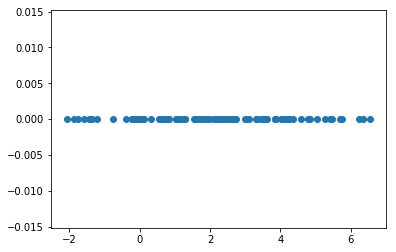
\includegraphics{images/fig2-1-3.png}
\caption{Example of a possible result}
\end{figure}

    \begin{tcolorbox}[breakable, size=fbox, boxrule=1pt, pad at break*=1mm,colback=cellbackground, colframe=cellborder]
\prompt{In}{incolor}{18}{\boxspacing}
\begin{Verbatim}[commandchars=\\\{\}]
\PY{k}{def} \PY{n+nf}{gen\PYZus{}samples}\PY{p}{(}\PY{n}{n}\PY{p}{,} \PY{n}{mu}\PY{p}{,} \PY{n}{sigma}\PY{p}{)}\PY{p}{:}
    \PY{l+s+sd}{\PYZdq{}\PYZdq{}\PYZdq{}Generate n samples of a gaussian distribution}
\PY{l+s+sd}{    }
\PY{l+s+sd}{    Args:}
\PY{l+s+sd}{        n: Number of samples}
\PY{l+s+sd}{        mu: mean of the distribution}
\PY{l+s+sd}{        sigma: standard deviation of the distribution}

\PY{l+s+sd}{    Returns:}
\PY{l+s+sd}{        array of samples}
\PY{l+s+sd}{    \PYZdq{}\PYZdq{}\PYZdq{}}
    
    \PY{n}{randomValues} \PY{o}{=} \PY{n}{np}\PY{o}{.}\PY{n}{random}\PY{o}{.}\PY{n}{randn}\PY{p}{(}\PY{n}{n}\PY{p}{)}
    \PY{n}{samples} \PY{o}{=} \PY{n}{sigma} \PY{o}{*} \PY{n}{randomValues} \PY{o}{+} \PY{n}{mu}
    \PY{k}{return} \PY{n}{samples}
\end{Verbatim}
\end{tcolorbox}

    \begin{tcolorbox}[breakable, size=fbox, boxrule=1pt, pad at break*=1mm,colback=cellbackground, colframe=cellborder]
\prompt{In}{incolor}{20}{\boxspacing}
\begin{Verbatim}[commandchars=\\\{\}]
\PY{c+c1}{\PYZsh{} RUN}
\PY{c+c1}{\PYZsh{} RUN}
\PY{n}{num} \PY{o}{=} \PY{l+m+mi}{100}
\PY{n}{mu} \PY{o}{=} \PY{l+m+mi}{2}
\PY{n}{sigma} \PY{o}{=} \PY{l+m+mi}{2}
\PY{n}{plt}\PY{o}{.}\PY{n}{scatter}\PY{p}{(}\PY{n}{gen\PYZus{}samples}\PY{p}{(}\PY{n}{num}\PY{p}{,} \PY{n}{mu}\PY{p}{,} \PY{n}{sigma}\PY{p}{)}\PY{p}{,} \PY{n}{np}\PY{o}{.}\PY{n}{zeros}\PY{p}{(}\PY{n}{num}\PY{p}{)}\PY{p}{)}
\PY{n}{plt}\PY{o}{.}\PY{n}{show}\PY{p}{(}\PY{p}{)}
\end{Verbatim}
\end{tcolorbox}

    \begin{center}
    \adjustimage{max size={0.9\linewidth}{0.9\paperheight}}{output_8_0.pdf}
    \end{center}
    { \hspace*{\fill} \\}
    
    \hypertarget{thinking-about-it-1}{%
\subsubsection{Thinking about it (1)}\label{thinking-about-it-1}}

Having completed the code above, you will be able to \textbf{answer the
following questions}:

\begin{itemize}
\item
  Which value do the samples concentrate around? Why?

  \(\mu\). Because mu is the mean of the distribution, so all values
  will be around the mean.
\item
  Why we observe less samples the further they are from that value?

  Because in those cases, \(\sigma*x\) (where x is the random value) has
  resulted a relatively high value respect to \(\mu\), which is why it
  moves away from it.
\end{itemize}

    Indeed, if we keep sampling the distribution and build an histogram of
the obtained samples, the resulting histogram will be similar to its
respective gaussian given a large enough number of samples.

    \hypertarget{assignment-3-building-an-histogram-of-samples}{%
\subsubsection{\texorpdfstring{\textbf{{ASSIGNMENT 3: Building an
histogram of
samples}}}{ASSIGNMENT 3: Building an histogram of samples}}\label{assignment-3-building-an-histogram-of-samples}}

For checking this, we ask you to:

\begin{enumerate}
\def\labelenumi{\arabic{enumi}.}
\item
  Create a large sample vector, i.e.~size 1000.
\item
  Then, complete the function \texttt{hist\_slice()}, which takes an
  array of samples and an integer \texttt{n}. This function plots the
  first \texttt{n} values of the array as a \textbf{histogram}.
\item
  To show the results of the exercise we will employ the use of Jupyter
  widgets. You can find more info about them here
  \href{https://ipywidgets.readthedocs.io/en/latest/index.html}{{[}link{]}},
  but for the time being use the commented call to \texttt{interact}.
\end{enumerate}

Play around with different parameters of the
\href{https://matplotlib.org/api/_as_gen/matplotlib.pyplot.hist.html?highlight=hist\#matplotlib.pyplot.hist}{\texttt{plt.hist()}}
function from matplotlib.

The bars of the histogram should be normalized by the total area. (HINT:
Set the optional \texttt{density} and \texttt{stacked} parameters of
\texttt{hist()} to True)

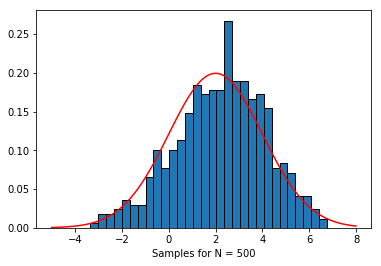
\includegraphics{images/fig2-1-4.png}

    \begin{tcolorbox}[breakable, size=fbox, boxrule=1pt, pad at break*=1mm,colback=cellbackground, colframe=cellborder]
\prompt{In}{incolor}{22}{\boxspacing}
\begin{Verbatim}[commandchars=\\\{\}]
\PY{k}{def} \PY{n+nf}{hist\PYZus{}slice}\PY{p}{(}\PY{n}{samples}\PY{p}{,} \PY{n}{n}\PY{p}{)}\PY{p}{:}
    \PY{l+s+sd}{\PYZdq{}\PYZdq{}\PYZdq{}Plot histogram for the first n values in samples\PYZdq{}\PYZdq{}\PYZdq{}}        
    \PY{n}{X} \PY{o}{=} \PY{n}{np}\PY{o}{.}\PY{n}{linspace}\PY{p}{(}\PY{o}{\PYZhy{}}\PY{l+m+mf}{5.}\PY{p}{,} \PY{l+m+mf}{8.}\PY{p}{,} \PY{l+m+mi}{100}\PY{p}{)}
    \PY{n}{mu} \PY{o}{=} \PY{l+m+mi}{2}
    \PY{n}{sigma} \PY{o}{=} \PY{l+m+mi}{2}
    \PY{n}{plt}\PY{o}{.}\PY{n}{plot}\PY{p}{(}\PY{n}{X}\PY{p}{,} \PY{n}{evaluate\PYZus{}gaussian}\PY{p}{(}\PY{n}{mu}\PY{p}{,} \PY{n}{sigma}\PY{p}{,} \PY{n}{X}\PY{p}{)}\PY{p}{,} \PY{l+s+s1}{\PYZsq{}}\PY{l+s+s1}{r}\PY{l+s+s1}{\PYZsq{}}\PY{p}{)}
    \PY{n}{plt}\PY{o}{.}\PY{n}{hist}\PY{p}{(}\PY{n}{samples}\PY{p}{[}\PY{l+m+mi}{0}\PY{p}{:}\PY{n}{n}\PY{p}{]}\PY{p}{,} \PY{n}{bins}\PY{o}{=}\PY{l+m+mi}{40}\PY{p}{,} \PY{n}{edgecolor}\PY{o}{=}\PY{p}{(}\PY{l+m+mi}{0}\PY{p}{,} \PY{l+m+mi}{0}\PY{p}{,} \PY{l+m+mi}{0}\PY{p}{)}\PY{p}{,} \PY{n}{density}\PY{o}{=}\PY{k+kc}{True}\PY{p}{,} \PY{n}{stacked}\PY{o}{=}\PY{k+kc}{True}\PY{p}{,} \PY{n}{color}\PY{o}{=}\PY{p}{(}\PY{l+m+mf}{0.1}\PY{p}{,}\PY{l+m+mi}{0}\PY{p}{,}\PY{l+m+mf}{0.3}\PY{p}{)}\PY{p}{)}    
    \PY{n}{plt}\PY{o}{.}\PY{n}{xlabel}\PY{p}{(}\PY{l+s+s2}{\PYZdq{}}\PY{l+s+s2}{Samples for N = }\PY{l+s+si}{\PYZpc{}d}\PY{l+s+s2}{\PYZdq{}} \PY{o}{\PYZpc{}} \PY{p}{(}\PY{n+nb}{len}\PY{p}{(}\PY{n}{samples}\PY{p}{)}\PY{p}{)}\PY{p}{)}
    \PY{n}{plt}\PY{o}{.}\PY{n}{show}\PY{p}{(}\PY{p}{)}
\end{Verbatim}
\end{tcolorbox}

    \begin{tcolorbox}[breakable, size=fbox, boxrule=1pt, pad at break*=1mm,colback=cellbackground, colframe=cellborder]
\prompt{In}{incolor}{24}{\boxspacing}
\begin{Verbatim}[commandchars=\\\{\}]
\PY{c+c1}{\PYZsh{} RUN}
\PY{n}{random}\PY{o}{.}\PY{n}{seed}\PY{p}{(}\PY{l+m+mi}{0}\PY{p}{)}
\PY{n}{samples} \PY{o}{=} \PY{n}{gen\PYZus{}samples}\PY{p}{(}\PY{l+m+mi}{500}\PY{p}{,} \PY{l+m+mi}{2}\PY{p}{,} \PY{l+m+mi}{2}\PY{p}{)}
\PY{n}{n} \PY{o}{=} \PY{l+m+mi}{5000}
\PY{n}{hist\PYZus{}slice}\PY{p}{(}\PY{n}{samples}\PY{p}{,} \PY{n}{n}\PY{p}{)}
\end{Verbatim}
\end{tcolorbox}

    \begin{center}
    \adjustimage{max size={0.9\linewidth}{0.9\paperheight}}{output_13_0.pdf}
    \end{center}
    { \hspace*{\fill} \\}
    
    \begin{tcolorbox}[breakable, size=fbox, boxrule=1pt, pad at break*=1mm,colback=cellbackground, colframe=cellborder]
\prompt{In}{incolor}{26}{\boxspacing}
\begin{Verbatim}[commandchars=\\\{\}]
\PY{c+c1}{\PYZsh{} RUN}
\PY{n}{interact}\PY{p}{(}\PY{n}{hist\PYZus{}slice}\PY{p}{,} \PY{n}{samples}\PY{o}{=}\PY{n}{fixed}\PY{p}{(}\PY{n}{samples}\PY{p}{)}\PY{p}{,} \PY{n}{n}\PY{o}{=}\PY{p}{(}\PY{l+m+mi}{100}\PY{p}{,} \PY{l+m+mi}{500}\PY{p}{,} \PY{l+m+mi}{100}\PY{p}{)}\PY{p}{)}
\end{Verbatim}
\end{tcolorbox}

    
    \begin{Verbatim}[commandchars=\\\{\}]
interactive(children=(IntSlider(value=300, description='n', max=500, min=100, step=100), Output()), \_dom\_class…
    \end{Verbatim}

    
            \begin{tcolorbox}[breakable, size=fbox, boxrule=.5pt, pad at break*=1mm, opacityfill=0]
\prompt{Out}{outcolor}{26}{\boxspacing}
\begin{Verbatim}[commandchars=\\\{\}]
<function \_\_main\_\_.hist\_slice(samples, n)>
\end{Verbatim}
\end{tcolorbox}
        
    \hypertarget{properties-of-the-gaussian-distribution}{%
\subsection{2.1.2 Properties of the Gaussian
distribution}\label{properties-of-the-gaussian-distribution}}

Once we have acquired a certain amount of familiarity with the gaussian
distribution, we can go along some of its principal properties, which
are the main reason of this distribution's wide usage in robotics.

    \begin{tcolorbox}[breakable, size=fbox, boxrule=1pt, pad at break*=1mm,colback=cellbackground, colframe=cellborder]
\prompt{In}{incolor}{28}{\boxspacing}
\begin{Verbatim}[commandchars=\\\{\}]
\PY{c+c1}{\PYZsh{} Imports}

\PY{k+kn}{from} \PY{n+nn}{scipy} \PY{k+kn}{import} \PY{n}{stats}
\PY{k+kn}{from} \PY{n+nn}{scipy} \PY{k+kn}{import} \PY{n}{signal}
\end{Verbatim}
\end{tcolorbox}

    \hypertarget{central-limit-theorem}{%
\subsubsection{Central limit theorem}\label{central-limit-theorem}}

\textbf{Property.} The sum of N independent and identically distributed
(i.i.d.) random variables, i.e.~that belong to the same distribution and
are independant to each other, becomes increasingly Gaussian the larger
is N.

This property holds true regardless of the probability distribution was
used to create the samples. It is one of the key concepts in
probability, as it allows the generalization of many problems.

You can see a video demonstration of this by running the cell bellow:

    \begin{tcolorbox}[breakable, size=fbox, boxrule=1pt, pad at break*=1mm,colback=cellbackground, colframe=cellborder]
\prompt{In}{incolor}{30}{\boxspacing}
\begin{Verbatim}[commandchars=\\\{\}]
\PY{o}{\PYZpc{}\PYZpc{}HTML}
\PY{p}{\PYZlt{}}\PY{n+nt}{center}\PY{p}{\PYZgt{}}
\PY{p}{\PYZlt{}}\PY{n+nt}{iframe} \PY{n+na}{width}\PY{o}{=}\PY{l+s}{\PYZdq{}560\PYZdq{}} \PY{n+na}{height}\PY{o}{=}\PY{l+s}{\PYZdq{}315\PYZdq{}} \PY{n+na}{src}\PY{o}{=}\PY{l+s}{\PYZdq{}https://www.youtube.com/embed/dlbkaurTAUg?autoplay=0\PYZam{}mute=1\PYZdq{}} \PY{n+na}{frameborder}\PY{o}{=}\PY{l+s}{\PYZdq{}0\PYZdq{}} \PY{n+na}{allow}\PY{o}{=}\PY{l+s}{\PYZdq{}accelerometer; autoplay; encrypted\PYZhy{}media; gyroscope; picture\PYZhy{}in\PYZhy{}picture\PYZdq{}} \PY{n+na}{allowfullscreen}\PY{p}{\PYZgt{}}\PY{p}{\PYZlt{}}\PY{p}{/}\PY{n+nt}{iframe}\PY{p}{\PYZgt{}}
\PY{p}{\PYZlt{}}\PY{p}{/}\PY{n+nt}{center}\PY{p}{\PYZgt{}}
\end{Verbatim}
\end{tcolorbox}

    
    \begin{Verbatim}[commandchars=\\\{\}]
<IPython.core.display.HTML object>
    \end{Verbatim}

    
    \hypertarget{assignment-4-verifying-the-central-limit-theorem}{%
\subsubsection{\texorpdfstring{\textbf{{ASSIGNMENT 4: Verifying the
central limit
theorem}}}{ASSIGNMENT 4: Verifying the central limit theorem}}\label{assignment-4-verifying-the-central-limit-theorem}}

We ask you to create a similar demonstration as the example above.

\begin{itemize}
\tightlist
\item
  Complete the following \texttt{plot\_sum\_demo} function. This
  function returns a vector of length \texttt{v\_length}, which results
  from the sum of \texttt{N} randomly generated vectors using an uniform
  distribution \([0, 1)\). Each random vector should have the same
  length (for example \texttt{v\_lenght=100}).
\item
  Inside the function, plot the corresponding histogram.
\item
  Finally, check that the resulting figure has the shape of a gaussian.
\end{itemize}

    \begin{tcolorbox}[breakable, size=fbox, boxrule=1pt, pad at break*=1mm,colback=cellbackground, colframe=cellborder]
\prompt{In}{incolor}{32}{\boxspacing}
\begin{Verbatim}[commandchars=\\\{\}]
\PY{k}{def} \PY{n+nf}{plot\PYZus{}sum}\PY{p}{(}\PY{n}{v\PYZus{}length}\PY{p}{,} \PY{n}{N}\PY{p}{)}\PY{p}{:}
    
    \PY{c+c1}{\PYZsh{}create the vector for storing the sums}
    \PY{n}{sum\PYZus{}samples} \PY{o}{=} \PY{n}{np}\PY{o}{.}\PY{n}{zeros}\PY{p}{(}\PY{n}{v\PYZus{}length}\PY{p}{)}
    
    \PY{c+c1}{\PYZsh{} Generate N vectors of samples and sum them within sum\PYZus{}samples}
    \PY{k}{for} \PY{n}{\PYZus{}} \PY{o+ow}{in} \PY{n+nb}{range}\PY{p}{(}\PY{l+m+mi}{0}\PY{p}{,} \PY{n}{N}\PY{p}{)}\PY{p}{:}
        \PY{n}{sum\PYZus{}samples} \PY{o}{+}\PY{o}{=} \PY{n}{random}\PY{o}{.}\PY{n}{rand}\PY{p}{(}\PY{n}{v\PYZus{}length}\PY{p}{)}
        
    \PY{c+c1}{\PYZsh{} Plot the resultant histogram    }
    \PY{n}{plt}\PY{o}{.}\PY{n}{hist}\PY{p}{(}\PY{n}{sum\PYZus{}samples}\PY{p}{,}
             \PY{n}{bins}\PY{o}{=}\PY{l+m+mi}{25}\PY{p}{,} \PY{n}{density}\PY{o}{=}\PY{k+kc}{True}\PY{p}{,}
             \PY{n}{stacked}\PY{o}{=}\PY{k+kc}{True}\PY{p}{,} \PY{n}{edgecolor}\PY{o}{=}\PY{l+s+s1}{\PYZsq{}}\PY{l+s+s1}{black}\PY{l+s+s1}{\PYZsq{}}\PY{p}{)}    
\end{Verbatim}
\end{tcolorbox}

    \begin{tcolorbox}[breakable, size=fbox, boxrule=1pt, pad at break*=1mm,colback=cellbackground, colframe=cellborder]
\prompt{In}{incolor}{34}{\boxspacing}
\begin{Verbatim}[commandchars=\\\{\}]
\PY{c+c1}{\PYZsh{} RUN}
\PY{n}{v\PYZus{}length} \PY{o}{=} \PY{l+m+mi}{1000}
\PY{n}{N} \PY{o}{=} \PY{l+m+mi}{10}
\PY{n}{plot\PYZus{}sum}\PY{p}{(}\PY{n}{v\PYZus{}length}\PY{p}{,} \PY{n}{N}\PY{p}{)}
\end{Verbatim}
\end{tcolorbox}

    \begin{center}
    \adjustimage{max size={0.9\linewidth}{0.9\paperheight}}{output_21_0.pdf}
    \end{center}
    { \hspace*{\fill} \\}
    
    Now play a bit with the number of randomly generated vectors

    \begin{tcolorbox}[breakable, size=fbox, boxrule=1pt, pad at break*=1mm,colback=cellbackground, colframe=cellborder]
\prompt{In}{incolor}{36}{\boxspacing}
\begin{Verbatim}[commandchars=\\\{\}]
\PY{n}{interact}\PY{p}{(}\PY{n}{plot\PYZus{}sum}\PY{p}{,} \PY{n}{v\PYZus{}length}\PY{o}{=}\PY{n}{fixed}\PY{p}{(}\PY{n}{v\PYZus{}length}\PY{p}{)}\PY{p}{,} \PY{n}{N}\PY{o}{=}\PY{p}{(}\PY{l+m+mi}{0}\PY{p}{,} \PY{l+m+mi}{25}\PY{p}{,} \PY{l+m+mi}{1}\PY{p}{)}\PY{p}{)}
\end{Verbatim}
\end{tcolorbox}

    
    \begin{Verbatim}[commandchars=\\\{\}]
interactive(children=(IntSlider(value=12, description='N', max=25), Output()), \_dom\_classes=('widget-interact'…
    \end{Verbatim}

    
            \begin{tcolorbox}[breakable, size=fbox, boxrule=.5pt, pad at break*=1mm, opacityfill=0]
\prompt{Out}{outcolor}{36}{\boxspacing}
\begin{Verbatim}[commandchars=\\\{\}]
<function \_\_main\_\_.plot\_sum(v\_length, N)>
\end{Verbatim}
\end{tcolorbox}
        
    \hypertarget{product-of-gaussians}{%
\subsubsection{Product of gaussians}\label{product-of-gaussians}}

The weighted sum of two gaussians, results in a random variable which
its the product of both. This product of 2 gaussians is defined as:

\[
     N\left(
        \frac{\sigma_2^2\mu_1+\sigma_1^2\mu_2}
        {\sigma_1^2+\sigma_2^2},
         \frac{\sigma_1^2 \sigma_ 2^2}
         {\sigma_1^2 + \sigma_ 2^2}
     \right)
\]

    \hypertarget{assignment-5-multiplying-gaussians}{%
\subsubsection{\texorpdfstring{\textbf{{ASSIGNMENT 5: Multiplying
gaussians}}}{ASSIGNMENT 5: Multiplying gaussians}}\label{assignment-5-multiplying-gaussians}}

Complete the following function to compute the product of two gaussians
distributions.

Draw the result and check that corresponds to the formula above playing
with different distributions.

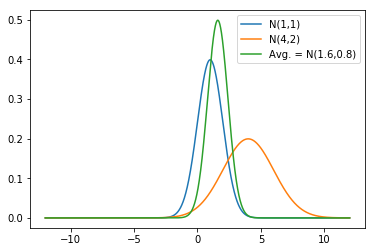
\includegraphics{images/fig2-2-3.png}

    \begin{tcolorbox}[breakable, size=fbox, boxrule=1pt, pad at break*=1mm,colback=cellbackground, colframe=cellborder]
\prompt{In}{incolor}{38}{\boxspacing}
\begin{Verbatim}[commandchars=\\\{\}]
\PY{k}{def} \PY{n+nf}{gaussians\PYZus{}product}\PY{p}{(}\PY{n}{mu1}\PY{p}{,}\PY{n}{mu2}\PY{p}{,}\PY{n}{sig1}\PY{p}{,}\PY{n}{sig2}\PY{p}{,}\PY{n}{x}\PY{p}{)}\PY{p}{:}
    
    \PY{n}{var1}\PY{p}{,} \PY{n}{var2} \PY{o}{=} \PY{n+nb}{pow}\PY{p}{(}\PY{n}{sig1}\PY{p}{,} \PY{l+m+mi}{2}\PY{p}{)}\PY{p}{,} \PY{n+nb}{pow}\PY{p}{(}\PY{n}{sig2}\PY{p}{,} \PY{l+m+mi}{2}\PY{p}{)} \PY{c+c1}{\PYZsh{} Get the variances from the standar deviations}

    \PY{n}{X} \PY{o}{=} \PY{n}{np}\PY{o}{.}\PY{n}{arange}\PY{p}{(}\PY{o}{\PYZhy{}}\PY{l+m+mi}{12}\PY{p}{,} \PY{l+m+mi}{12}\PY{p}{,} \PY{l+m+mi}{1}\PY{o}{/}\PY{n}{x}\PY{p}{)}
    \PY{n}{pdf1} \PY{o}{=} \PY{n}{stats}\PY{o}{.}\PY{n}{norm}\PY{p}{(}\PY{n}{loc}\PY{o}{=}\PY{n}{mu1}\PY{p}{,} \PY{n}{scale}\PY{o}{=}\PY{n}{sig1}\PY{p}{)}\PY{o}{.}\PY{n}{pdf}\PY{p}{(}\PY{n}{X}\PY{p}{)}
    \PY{n}{pdf2} \PY{o}{=} \PY{n}{stats}\PY{o}{.}\PY{n}{norm}\PY{p}{(}\PY{n}{loc}\PY{o}{=}\PY{n}{mu2}\PY{p}{,} \PY{n}{scale}\PY{o}{=}\PY{n}{sig2}\PY{p}{)}\PY{o}{.}\PY{n}{pdf}\PY{p}{(}\PY{n}{X}\PY{p}{)}

    \PY{n}{plt}\PY{o}{.}\PY{n}{plot}\PY{p}{(}\PY{n}{X}\PY{p}{,} \PY{n}{pdf1}\PY{p}{,} \PY{n}{label}\PY{o}{=}\PY{l+s+s1}{\PYZsq{}}\PY{l+s+s1}{N(}\PY{l+s+si}{\PYZob{}\PYZcb{}}\PY{l+s+s1}{,}\PY{l+s+si}{\PYZob{}\PYZcb{}}\PY{l+s+s1}{)}\PY{l+s+s1}{\PYZsq{}}\PY{o}{.}\PY{n}{format}\PY{p}{(}\PY{n}{mu1}\PY{p}{,} \PY{n}{sig1}\PY{p}{)}\PY{p}{)}
    \PY{n}{plt}\PY{o}{.}\PY{n}{plot}\PY{p}{(}\PY{n}{X}\PY{p}{,} \PY{n}{pdf2}\PY{p}{,} \PY{n}{label}\PY{o}{=}\PY{l+s+s1}{\PYZsq{}}\PY{l+s+s1}{N(}\PY{l+s+si}{\PYZob{}\PYZcb{}}\PY{l+s+s1}{,}\PY{l+s+si}{\PYZob{}\PYZcb{}}\PY{l+s+s1}{)}\PY{l+s+s1}{\PYZsq{}}\PY{o}{.}\PY{n}{format}\PY{p}{(}\PY{n}{mu2}\PY{p}{,} \PY{n}{sig2}\PY{p}{)}\PY{p}{)}

    
    \PY{c+c1}{\PYZsh{} Get the parameters defining the gaussian distribution resulting from their product}
    \PY{n}{mu3} \PY{o}{=} \PY{p}{(}\PY{p}{(}\PY{n}{var2}\PY{o}{*}\PY{n}{mu1}\PY{p}{)} \PY{o}{+} \PY{p}{(}\PY{n}{var1}\PY{o}{*}\PY{n}{mu2}\PY{p}{)}\PY{p}{)}\PY{o}{/}\PY{p}{(}\PY{n}{var1}\PY{o}{+}\PY{n}{var2}\PY{p}{)}
    \PY{n}{sig3} \PY{o}{=} \PY{p}{(}\PY{n}{var1}\PY{o}{*}\PY{n}{var2}\PY{p}{)}\PY{o}{/}\PY{p}{(}\PY{n}{var1}\PY{o}{+}\PY{n}{var2}\PY{p}{)}
    \PY{n}{c} \PY{o}{=} \PY{n}{stats}\PY{o}{.}\PY{n}{norm}\PY{p}{(}\PY{n}{loc}\PY{o}{=}\PY{n}{mu3}\PY{p}{,} \PY{n}{scale}\PY{o}{=}\PY{n}{sig3}\PY{p}{)}\PY{o}{.}\PY{n}{pdf}\PY{p}{(}\PY{n}{X}\PY{p}{)}

    \PY{n}{plt}\PY{o}{.}\PY{n}{plot}\PY{p}{(}\PY{n}{X}\PY{p}{,} \PY{n}{c}\PY{p}{,} \PY{n}{label}\PY{o}{=}\PY{l+s+s1}{\PYZsq{}}\PY{l+s+s1}{Avg. = N(}\PY{l+s+si}{\PYZob{}\PYZcb{}}\PY{l+s+s1}{,}\PY{l+s+si}{\PYZob{}\PYZcb{}}\PY{l+s+s1}{)}\PY{l+s+s1}{\PYZsq{}}\PY{o}{.}\PY{n}{format}\PY{p}{(}\PY{n}{mu3}\PY{p}{,} \PY{n}{sig3}\PY{p}{)}\PY{p}{)}
    \PY{n}{plt}\PY{o}{.}\PY{n}{legend}\PY{p}{(}\PY{p}{)}


    
    
\end{Verbatim}
\end{tcolorbox}

    \begin{tcolorbox}[breakable, size=fbox, boxrule=1pt, pad at break*=1mm,colback=cellbackground, colframe=cellborder]
\prompt{In}{incolor}{40}{\boxspacing}
\begin{Verbatim}[commandchars=\\\{\}]
\PY{n}{mu1}\PY{p}{,} \PY{n}{sig1} \PY{o}{=} \PY{l+m+mi}{1}\PY{p}{,} \PY{l+m+mi}{1}
\PY{n}{mu2}\PY{p}{,} \PY{n}{sig2} \PY{o}{=} \PY{l+m+mi}{4}\PY{p}{,} \PY{l+m+mi}{2}
\PY{n}{x} \PY{o}{=} \PY{l+m+mi}{1000}    

\PY{n}{gaussians\PYZus{}product}\PY{p}{(}\PY{n}{mu1}\PY{p}{,}\PY{n}{mu2}\PY{p}{,}\PY{n}{sig1}\PY{p}{,}\PY{n}{sig2}\PY{p}{,}\PY{n}{x}\PY{p}{)}
\end{Verbatim}
\end{tcolorbox}

    \begin{center}
    \adjustimage{max size={0.9\linewidth}{0.9\paperheight}}{output_27_0.pdf}
    \end{center}
    { \hspace*{\fill} \\}
    
    \hypertarget{linear-transformation-of-gaussian-random-variables.}{%
\subsubsection{Linear transformation of gaussian random
variables.}\label{linear-transformation-of-gaussian-random-variables.}}

\textbf{Property.} The gaussian distributions are closed under linear
transformations, i.e.~when we apply a sum or product to normal random
variables, the result is also a normal random variable.

This is also a remarkable property, for example in the field of robotics
we can \emph{operate normally over random distributions} as long as we
only use linear functions. Otherwise, if we are in need to apply a
\emph{non-linear transformation} (e.g.~sine, cosine, \ldots), the
resulting probability distribution \emph{will not correspond to any
Gaussian pdf}, causing additional complications in the process.

    \hypertarget{assignment-6-applying-linear-transformations}{%
\subsubsection{\texorpdfstring{\textbf{{ASSIGNMENT 6: Applying linear
transformations}}}{ASSIGNMENT 6: Applying linear transformations}}\label{assignment-6-applying-linear-transformations}}

\begin{itemize}
\tightlist
\item
  Generate a number \texttt{n\_samples} of random samples from the dist.
  \(N(1,1)\).
\item
  Then transform it following the expression \(y = a*x + b\) and plot
  the result for \(a=b=2\).
\item
  Finally, draw on top the pdf of \(N(4,4)\) and check that both are the
  same.
\end{itemize}

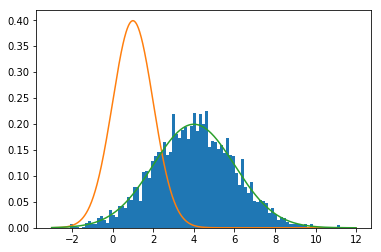
\includegraphics{images/fig2-2-4.png}

    \begin{tcolorbox}[breakable, size=fbox, boxrule=1pt, pad at break*=1mm,colback=cellbackground, colframe=cellborder]
\prompt{In}{incolor}{41}{\boxspacing}
\begin{Verbatim}[commandchars=\\\{\}]
\PY{k}{def} \PY{n+nf}{linear\PYZus{}transformation}\PY{p}{(}\PY{n}{n\PYZus{}samples}\PY{p}{,} \PY{n}{a}\PY{p}{,} \PY{n}{b}\PY{p}{)}\PY{p}{:}
    \PY{l+s+sd}{\PYZdq{}\PYZdq{}\PYZdq{}Apply lineal transform. Generating n\PYZus{}samples samples from N(1,1)\PYZdq{}\PYZdq{}\PYZdq{}}
    
    \PY{c+c1}{\PYZsh{} Generates n\PYZus{}samples from N(1,1)}
    \PY{n}{mu} \PY{o}{=} \PY{l+m+mi}{1}
    \PY{n}{stdv} \PY{o}{=} \PY{l+m+mi}{1}
    \PY{n}{samples} \PY{o}{=} \PY{n}{stats}\PY{o}{.}\PY{n}{norm}\PY{p}{(}\PY{n}{loc}\PY{o}{=}\PY{n}{mu}\PY{p}{,} \PY{n}{scale}\PY{o}{=}\PY{n}{stdv}\PY{p}{)}\PY{o}{.}\PY{n}{rvs}\PY{p}{(}\PY{n}{n\PYZus{}samples}\PY{p}{)}
    
    \PY{n}{samples\PYZus{}2} \PY{o}{=} \PY{n}{samples}\PY{o}{*}\PY{n}{a} \PY{o}{+} \PY{n}{b} \PY{c+c1}{\PYZsh{} Apply the linear transformation to the samples}

    \PY{c+c1}{\PYZsh{} Plot histogram (blue bars)}
    \PY{n}{n}\PY{p}{,} \PY{n}{bins}\PY{p}{,} \PY{n}{patches} \PY{o}{=} \PY{n}{plt}\PY{o}{.}\PY{n}{hist}\PY{p}{(}\PY{n}{samples\PYZus{}2}\PY{p}{,} \PY{n}{bins}\PY{o}{=}\PY{l+m+mi}{90}\PY{p}{,} \PY{n}{density}\PY{o}{=}\PY{k+kc}{True}\PY{p}{,} \PY{n}{stacked}\PY{o}{=}\PY{k+kc}{True}\PY{p}{)}

    \PY{n}{delta} \PY{o}{=} \PY{l+m+mi}{1}\PY{o}{/}\PY{n}{samples}\PY{o}{.}\PY{n}{size} 
    \PY{n}{X} \PY{o}{=} \PY{n}{np}\PY{o}{.}\PY{n}{arange}\PY{p}{(}\PY{n}{bins}\PY{p}{[}\PY{l+m+mi}{0}\PY{p}{]}\PY{p}{,} \PY{n}{bins}\PY{p}{[}\PY{o}{\PYZhy{}}\PY{l+m+mi}{1}\PY{p}{]}\PY{p}{,} \PY{n}{delta}\PY{p}{)}
    \PY{n}{A} \PY{o}{=} \PY{n}{stats}\PY{o}{.}\PY{n}{norm}\PY{p}{(}\PY{n}{loc}\PY{o}{=}\PY{l+m+mi}{1}\PY{p}{,} \PY{n}{scale}\PY{o}{=}\PY{l+m+mi}{1}\PY{p}{)}\PY{o}{.}\PY{n}{pdf}\PY{p}{(}\PY{n}{X}\PY{p}{)} \PY{c+c1}{\PYZsh{} Evaluate N(1,1) in X}
    \PY{n}{B} \PY{o}{=} \PY{n}{stats}\PY{o}{.}\PY{n}{norm}\PY{p}{(}\PY{n}{loc}\PY{o}{=}\PY{n}{a}\PY{o}{*}\PY{n}{mu}\PY{o}{+}\PY{n}{b}\PY{p}{,} \PY{n}{scale}\PY{o}{=}\PY{n}{stdv}\PY{o}{*}\PY{n}{a}\PY{p}{)}\PY{o}{.}\PY{n}{pdf}\PY{p}{(}\PY{n}{X}\PY{p}{)} \PY{c+c1}{\PYZsh{} Evaluate the resultant distribution in X}
    
    \PY{c+c1}{\PYZsh{} Show results}
    \PY{n}{plt}\PY{o}{.}\PY{n}{plot}\PY{p}{(}\PY{n}{X}\PY{p}{,} \PY{n}{A}\PY{p}{,} \PY{n}{color}\PY{o}{=}\PY{l+s+s1}{\PYZsq{}}\PY{l+s+s1}{red}\PY{l+s+s1}{\PYZsq{}}\PY{p}{,} \PY{n}{label}\PY{o}{=}\PY{l+s+s1}{\PYZsq{}}\PY{l+s+s1}{N(}\PY{l+s+si}{\PYZob{}\PYZcb{}}\PY{l+s+s1}{,}\PY{l+s+si}{\PYZob{}\PYZcb{}}\PY{l+s+s1}{)}\PY{l+s+s1}{\PYZsq{}}\PY{o}{.}\PY{n}{format}\PY{p}{(}\PY{n}{mu}\PY{p}{,} \PY{n}{stdv}\PY{p}{)}\PY{p}{)}
    \PY{n}{plt}\PY{o}{.}\PY{n}{plot}\PY{p}{(}\PY{n}{X}\PY{p}{,} \PY{n}{B}\PY{p}{,} \PY{n}{color}\PY{o}{=}\PY{l+s+s1}{\PYZsq{}}\PY{l+s+s1}{green}\PY{l+s+s1}{\PYZsq{}}\PY{p}{,} \PY{n}{label}\PY{o}{=}\PY{l+s+s1}{\PYZsq{}}\PY{l+s+s1}{N(}\PY{l+s+si}{\PYZob{}\PYZcb{}}\PY{l+s+s1}{,}\PY{l+s+si}{\PYZob{}\PYZcb{}}\PY{l+s+s1}{)}\PY{l+s+s1}{\PYZsq{}}\PY{o}{.}\PY{n}{format}\PY{p}{(}\PY{n}{a}\PY{o}{*}\PY{n}{mu}\PY{o}{+}\PY{n}{b}\PY{p}{,} \PY{n}{stdv}\PY{o}{*}\PY{n}{a}\PY{p}{)}\PY{p}{)}
    \PY{n}{plt}\PY{o}{.}\PY{n}{legend}\PY{p}{(}\PY{p}{)}
\end{Verbatim}
\end{tcolorbox}

    \begin{tcolorbox}[breakable, size=fbox, boxrule=1pt, pad at break*=1mm,colback=cellbackground, colframe=cellborder]
\prompt{In}{incolor}{42}{\boxspacing}
\begin{Verbatim}[commandchars=\\\{\}]
\PY{c+c1}{\PYZsh{} RUN}
\PY{n}{n\PYZus{}samples} \PY{o}{=} \PY{l+m+mi}{3000}
\PY{n}{a} \PY{o}{=} \PY{l+m+mi}{2}
\PY{n}{b} \PY{o}{=} \PY{l+m+mi}{2}
\PY{n}{linear\PYZus{}transformation}\PY{p}{(}\PY{n}{n\PYZus{}samples}\PY{p}{,} \PY{n}{a}\PY{p}{,} \PY{n}{b}\PY{p}{)}
\end{Verbatim}
\end{tcolorbox}

    \begin{center}
    \adjustimage{max size={0.9\linewidth}{0.9\paperheight}}{output_31_0.pdf}
    \end{center}
    { \hspace*{\fill} \\}
    
    Now play a bit with different values for \(a\) and \(b\).

    \begin{tcolorbox}[breakable, size=fbox, boxrule=1pt, pad at break*=1mm,colback=cellbackground, colframe=cellborder]
\prompt{In}{incolor}{43}{\boxspacing}
\begin{Verbatim}[commandchars=\\\{\}]
\PY{n}{interact}\PY{p}{(}\PY{n}{linear\PYZus{}transformation}\PY{p}{,} \PY{n}{n\PYZus{}samples}\PY{o}{=}\PY{n}{fixed}\PY{p}{(}\PY{n}{n\PYZus{}samples}\PY{p}{)}\PY{p}{,} \PY{n}{b}\PY{o}{=}\PY{p}{(}\PY{o}{\PYZhy{}}\PY{l+m+mi}{5}\PY{p}{,} \PY{l+m+mi}{5}\PY{p}{,} \PY{l+m+mi}{1}\PY{p}{)}\PY{p}{,} \PY{n}{a}\PY{o}{=}\PY{p}{(}\PY{l+m+mi}{1}\PY{p}{,} \PY{l+m+mi}{10}\PY{p}{,} \PY{l+m+mi}{1}\PY{p}{)}\PY{p}{)}
\end{Verbatim}
\end{tcolorbox}

    
    \begin{Verbatim}[commandchars=\\\{\}]
interactive(children=(IntSlider(value=5, description='a', max=10, min=1), IntSlider(value=0, description='b', …
    \end{Verbatim}

    
            \begin{tcolorbox}[breakable, size=fbox, boxrule=.5pt, pad at break*=1mm, opacityfill=0]
\prompt{Out}{outcolor}{43}{\boxspacing}
\begin{Verbatim}[commandchars=\\\{\}]
<function \_\_main\_\_.linear\_transformation(n\_samples, a, b)>
\end{Verbatim}
\end{tcolorbox}
        
    \hypertarget{bidimensional-normal-distribution}{%
\subsection{2.1.3 Bidimensional normal
distribution}\label{bidimensional-normal-distribution}}

Most useful applications of gaussian distributions does not only look at
individual distributions or variables, but an assortment of random
distributions which can be dependant to each other. Some examples of
these \emph{multidimensional distributions} we will use in following
exercises are: the pose of a robot \((x, y, \theta)\), an observation
from a series of range sensors \(([z_0, z_1, \dots, z_n])\), among
others.

In the specific case of Gaussian distributions they present certain key
differences:

\begin{itemize}
\tightlist
\item
  The \emph{mean} \((\mu)\) now it contains a vector of \(n\) values
  \(([\mu_1, \mu_2, \dots, \mu_n]')\). Its dimensionality/shape is
  \((n \times 1)\), i.e.~is a vertical vector.
\item
  The \emph{covariance} (now referred as \(\Sigma\)) is a full-blown
  matrix of shape \((n \times n)\). The case being, now we need to
  express the relations (i.e.~dependence) of each variable to the rest.
\end{itemize}

    \begin{tcolorbox}[breakable, size=fbox, boxrule=1pt, pad at break*=1mm,colback=cellbackground, colframe=cellborder]
\prompt{In}{incolor}{44}{\boxspacing}
\begin{Verbatim}[commandchars=\\\{\}]
\PY{c+c1}{\PYZsh{} Imports}
\PY{k+kn}{from} \PY{n+nn}{numpy} \PY{k+kn}{import} \PY{n}{linalg}
\PY{k+kn}{import} \PY{n+nn}{sys}
\PY{n}{sys}\PY{o}{.}\PY{n}{path}\PY{o}{.}\PY{n}{append}\PY{p}{(}\PY{l+s+s2}{\PYZdq{}}\PY{l+s+s2}{..}\PY{l+s+s2}{\PYZdq{}}\PY{p}{)}
\PY{k+kn}{from} \PY{n+nn}{utils}\PY{n+nn}{.}\PY{n+nn}{PlotEllipse} \PY{k+kn}{import} \PY{n}{PlotEllipse}
\end{Verbatim}
\end{tcolorbox}

    \hypertarget{sum-of-bidimensional-random-variables}{%
\subsection{Sum of bidimensional random
variables}\label{sum-of-bidimensional-random-variables}}

In this exercise, we will take a look at how gaussians behave when we
sum 2 multidimensional random variables (\emph{RV}).

Given the sum of 2 multidimensional gaussian RVs \((X_1, X_2)\), the
resulting RV \((X_3)\) also follows a gaussian distribution defined as:

\[
    \left.
    \begin{aligned}
    X_1 &\sim N(\mu_1, \Sigma_1) \\
    X_2 &\sim N(\mu_2, \Sigma_2) \\
    X_3 &= X_1 + X_2
    \end{aligned}
    \enspace\right\}\enspace 
    X_3 \sim N(\mu_1 + \mu_2, \Sigma_1 + \Sigma_2)
\]

    \hypertarget{assignment-7-summing-linear-transformations}{%
\subsubsection{\texorpdfstring{\textbf{{ASSIGNMENT 7: Summing linear
transformations}}}{ASSIGNMENT 7: Summing linear transformations}}\label{assignment-7-summing-linear-transformations}}

\begin{enumerate}
\def\labelenumi{\arabic{enumi}.}
\tightlist
\item
  Generate and draw \texttt{n\_samples} random samples from 2 different
  bidimensional dists. \(N_1=N(\mu_1,\Sigma_1)\) y
  \(N_2=N(\mu_2,\Sigma_2)\). The \emph{mean} \((\mu_n)\) is a vector of
  dimension \((2 \times 1)\) and the \emph{covariance} \((\sigma_n)\) a
  matrix \((2 \times 2)\). They represent the mean and covariance of
  each dist. respectively. Use the function
  \texttt{multivariate\_normal} from the module \textbf{scipy.stats}.
\item
  Draw both ellipses associated with each distribution. Use
  \texttt{PlotEllipse()} from the utils library that comes with these
  notebooks.
\item
  Sum both samples and draw the ellipse
  \(x_3 \sim N(\mu_1+\mu_2, \Sigma_1+\Sigma_2)\)
\end{enumerate}

WARN: When passing the mean to the \texttt{PlotEllipse()} function, it
takes a vector \((2 \times 1)\), whereas \texttt{multivariate\_normal()}
takes a flat array \((1 \times 2).\)

\textbf{Example}

Results for an example:

\begin{Shaded}
\begin{Highlighting}[]
\NormalTok{    n\_samples }\OperatorTok{=} \DecValTok{500}
    
\NormalTok{    mean1 }\OperatorTok{=}\NormalTok{ np.vstack([}\DecValTok{1}\NormalTok{, }\DecValTok{0}\NormalTok{])}
\NormalTok{    sigma1 }\OperatorTok{=}\NormalTok{ np.array([[}\DecValTok{3}\NormalTok{, }\DecValTok{2}\NormalTok{], [}\DecValTok{2}\NormalTok{, }\DecValTok{3}\NormalTok{]])}
\NormalTok{    mean2 }\OperatorTok{=}\NormalTok{ np.vstack([}\DecValTok{2}\NormalTok{, }\DecValTok{3}\NormalTok{])}
\NormalTok{    sigma2 }\OperatorTok{=}\NormalTok{ np.array([[}\DecValTok{2}\NormalTok{, }\DecValTok{0}\NormalTok{], [}\DecValTok{0}\NormalTok{, }\DecValTok{1}\NormalTok{]]) }
\end{Highlighting}
\end{Shaded}

\begin{figure}
\centering
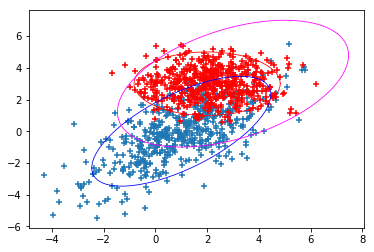
\includegraphics{images/fig2-3-1.png}
\caption{Example of a possible result}
\end{figure}

Fig. 1: Distribution of the sum of two RVs (in blue and red)

    \begin{tcolorbox}[breakable, size=fbox, boxrule=1pt, pad at break*=1mm,colback=cellbackground, colframe=cellborder]
\prompt{In}{incolor}{47}{\boxspacing}
\begin{Verbatim}[commandchars=\\\{\}]
\PY{k}{def} \PY{n+nf}{sum\PYZus{}of\PYZus{}rvs}\PY{p}{(}\PY{n}{mean1}\PY{p}{,}\PY{n}{sigma1}\PY{p}{,}\PY{n}{mean2}\PY{p}{,}\PY{n}{sigma2}\PY{p}{,}\PY{n}{n\PYZus{}samples}\PY{p}{)}\PY{p}{:}
    
    \PY{n}{fig}\PY{p}{,} \PY{n}{ax} \PY{o}{=} \PY{n}{plt}\PY{o}{.}\PY{n}{subplots}\PY{p}{(}\PY{p}{)}

    \PY{c+c1}{\PYZsh{} Build the normal distributions}
    \PY{n}{pdf1} \PY{o}{=} \PY{n}{stats}\PY{o}{.}\PY{n}{multivariate\PYZus{}normal}\PY{p}{(}\PY{n}{mean}\PY{o}{=}\PY{n}{mean1}\PY{o}{.}\PY{n}{flatten}\PY{p}{(}\PY{p}{)}\PY{p}{,} \PY{n}{cov}\PY{o}{=}\PY{n}{sigma1}\PY{p}{)} \PY{c+c1}{\PYZsh{} Hint: you have to use .flatten()}
    \PY{n}{pdf2} \PY{o}{=} \PY{n}{stats}\PY{o}{.}\PY{n}{multivariate\PYZus{}normal}\PY{p}{(}\PY{n}{mean}\PY{o}{=}\PY{n}{mean2}\PY{o}{.}\PY{n}{flatten}\PY{p}{(}\PY{p}{)}\PY{p}{,} \PY{n}{cov}\PY{o}{=}\PY{n}{sigma2}\PY{p}{)}

    \PY{c+c1}{\PYZsh{} Generate n\PYZus{}samples from them}
    \PY{n}{rvs1} \PY{o}{=} \PY{n}{pdf1}\PY{o}{.}\PY{n}{rvs}\PY{p}{(}\PY{n}{n\PYZus{}samples}\PY{p}{)}
    \PY{n}{rvs2} \PY{o}{=} \PY{n}{pdf2}\PY{o}{.}\PY{n}{rvs}\PY{p}{(}\PY{n}{n\PYZus{}samples}\PY{p}{)}

    \PY{c+c1}{\PYZsh{} Draw samples as crosses}
    \PY{n}{plt}\PY{o}{.}\PY{n}{scatter}\PY{p}{(}\PY{n}{rvs1}\PY{p}{[}\PY{p}{:}\PY{p}{,}\PY{l+m+mi}{0}\PY{p}{]}\PY{p}{,}\PY{n}{rvs1}\PY{p}{[}\PY{p}{:}\PY{p}{,}\PY{l+m+mi}{1}\PY{p}{]}\PY{p}{,} \PY{n}{marker}\PY{o}{=}\PY{l+s+s1}{\PYZsq{}}\PY{l+s+s1}{+}\PY{l+s+s1}{\PYZsq{}}\PY{p}{,} \PY{n}{color}\PY{o}{=}\PY{l+s+s1}{\PYZsq{}}\PY{l+s+s1}{blue}\PY{l+s+s1}{\PYZsq{}}\PY{p}{,} \PY{n}{label}\PY{o}{=}\PY{l+s+s2}{\PYZdq{}}\PY{l+s+s2}{N1}\PY{l+s+s2}{\PYZdq{}}\PY{p}{)}
    \PY{n}{plt}\PY{o}{.}\PY{n}{scatter}\PY{p}{(}\PY{n}{rvs2}\PY{p}{[}\PY{p}{:}\PY{p}{,}\PY{l+m+mi}{0}\PY{p}{]}\PY{p}{,}\PY{n}{rvs2}\PY{p}{[}\PY{p}{:}\PY{p}{,}\PY{l+m+mi}{1}\PY{p}{]}\PY{p}{,} \PY{n}{marker}\PY{o}{=}\PY{l+s+s1}{\PYZsq{}}\PY{l+s+s1}{+}\PY{l+s+s1}{\PYZsq{}}\PY{p}{,} \PY{n}{color}\PY{o}{=}\PY{l+s+s1}{\PYZsq{}}\PY{l+s+s1}{red}\PY{l+s+s1}{\PYZsq{}}\PY{p}{,} \PY{n}{label}\PY{o}{=}\PY{l+s+s2}{\PYZdq{}}\PY{l+s+s2}{N2}\PY{l+s+s2}{\PYZdq{}}\PY{p}{)}

    \PY{c+c1}{\PYZsh{} Draw ellipses \PYZsh{}}
    \PY{n}{mult} \PY{o}{=} \PY{l+m+mi}{2}
    \PY{n}{PlotEllipse}\PY{p}{(}\PY{n}{fig}\PY{p}{,} \PY{n}{ax}\PY{p}{,} \PY{n}{mean1}\PY{p}{,} \PY{n}{sigma1}\PY{p}{,} \PY{n}{mult}\PY{p}{,} \PY{n}{color}\PY{o}{=}\PY{l+s+s1}{\PYZsq{}}\PY{l+s+s1}{blue}\PY{l+s+s1}{\PYZsq{}}\PY{p}{)}
    \PY{n}{PlotEllipse}\PY{p}{(}\PY{n}{fig}\PY{p}{,} \PY{n}{ax}\PY{p}{,} \PY{n}{mean2}\PY{p}{,} \PY{n}{sigma2}\PY{p}{,} \PY{n}{mult}\PY{p}{,} \PY{n}{color}\PY{o}{=}\PY{l+s+s1}{\PYZsq{}}\PY{l+s+s1}{red}\PY{l+s+s1}{\PYZsq{}}\PY{p}{)}

    \PY{c+c1}{\PYZsh{} Compute and draw N1 + N2}
    \PY{n}{mean3Flatted} \PY{o}{=} \PY{n}{mean1} \PY{o}{+} \PY{n}{mean2}
    \PY{n}{sigma3} \PY{o}{=} \PY{n}{sigma1}\PY{o}{+}\PY{n}{sigma2}
    
    \PY{n}{rvs3} \PY{o}{=} \PY{n}{stats}\PY{o}{.}\PY{n}{multivariate\PYZus{}normal}\PY{p}{(}\PY{n}{mean}\PY{o}{=}\PY{n}{mean3Flatted}\PY{o}{.}\PY{n}{flatten}\PY{p}{(}\PY{p}{)}\PY{p}{,} \PY{n}{cov}\PY{o}{=}\PY{n}{sigma3}\PY{p}{)}\PY{o}{.}\PY{n}{rvs}\PY{p}{(}\PY{n}{n\PYZus{}samples}\PY{p}{)}
    \PY{c+c1}{\PYZsh{} plt.scatter(rvs3[:,0],rvs3[:,1], marker=\PYZsq{}+\PYZsq{},color=\PYZsq{}magenta\PYZsq{}, label=\PYZdq{}N1+N2\PYZdq{})}
    \PY{c+c1}{\PYZsh{} Esta linea esta comentada para que se asemeje al ejemplo superior, pero representa la suma de los valores y podria \PYZdq{}descomentarse\PYZdq{}}
    \PY{n}{PlotEllipse}\PY{p}{(}\PY{n}{fig}\PY{p}{,} \PY{n}{ax}\PY{p}{,} \PY{n}{mean3Flatted}\PY{p}{,} \PY{n}{sigma3}\PY{p}{,} \PY{n}{mult}\PY{p}{,} \PY{n}{color}\PY{o}{=}\PY{l+s+s1}{\PYZsq{}}\PY{l+s+s1}{magenta}\PY{l+s+s1}{\PYZsq{}}\PY{p}{)}
    \PY{n}{plt}\PY{o}{.}\PY{n}{legend}\PY{p}{(}\PY{p}{)}
\end{Verbatim}
\end{tcolorbox}

    \begin{tcolorbox}[breakable, size=fbox, boxrule=1pt, pad at break*=1mm,colback=cellbackground, colframe=cellborder]
\prompt{In}{incolor}{48}{\boxspacing}
\begin{Verbatim}[commandchars=\\\{\}]
\PY{n}{n\PYZus{}samples} \PY{o}{=} \PY{l+m+mi}{500}
\PY{n}{mean1} \PY{o}{=} \PY{n}{np}\PY{o}{.}\PY{n}{vstack}\PY{p}{(}\PY{p}{[}\PY{l+m+mi}{1}\PY{p}{,} \PY{l+m+mi}{0}\PY{p}{]}\PY{p}{)}
\PY{n}{sigma1} \PY{o}{=} \PY{n}{np}\PY{o}{.}\PY{n}{array}\PY{p}{(}\PY{p}{[}\PY{p}{[}\PY{l+m+mi}{3}\PY{p}{,} \PY{l+m+mi}{2}\PY{p}{]}\PY{p}{,} \PY{p}{[}\PY{l+m+mi}{2}\PY{p}{,} \PY{l+m+mi}{3}\PY{p}{]}\PY{p}{]}\PY{p}{)}
\PY{n}{mean2} \PY{o}{=} \PY{n}{np}\PY{o}{.}\PY{n}{vstack}\PY{p}{(}\PY{p}{[}\PY{l+m+mi}{2}\PY{p}{,} \PY{l+m+mi}{3}\PY{p}{]}\PY{p}{)}
\PY{n}{sigma2} \PY{o}{=} \PY{n}{np}\PY{o}{.}\PY{n}{array}\PY{p}{(}\PY{p}{[}\PY{p}{[}\PY{l+m+mi}{2}\PY{p}{,} \PY{l+m+mi}{0}\PY{p}{]}\PY{p}{,} \PY{p}{[}\PY{l+m+mi}{0}\PY{p}{,} \PY{l+m+mi}{1}\PY{p}{]}\PY{p}{]}\PY{p}{)}

\PY{n}{sum\PYZus{}of\PYZus{}rvs}\PY{p}{(}\PY{n}{mean1}\PY{p}{,}\PY{n}{sigma1}\PY{p}{,}\PY{n}{mean2}\PY{p}{,}\PY{n}{sigma2}\PY{p}{,}\PY{n}{n\PYZus{}samples}\PY{p}{)}
\end{Verbatim}
\end{tcolorbox}

    \begin{center}
    \adjustimage{max size={0.9\linewidth}{0.9\paperheight}}{output_39_0.pdf}
    \end{center}
    { \hspace*{\fill} \\}
    
    \hypertarget{product-of-gaussian-pdfs}{%
\subsection{Product of gaussian pdfs}\label{product-of-gaussian-pdfs}}

The product of two gaussian distributions (\emph{pdfs}) is also a
gaussian distribution. This distribution corresponds to the weighted
mean of samples from that same \emph{pdfs}.

Given two gaussian distributions \(N_1 \sim N(\mu_1, \Sigma_1)\) and
\(N_2 \sim N(\mu_2, \Sigma_2)\), the resulting gaussian \(N_3\) is
defined as:

\[
\begin{equation}
    \Sigma_3 = (\Sigma_1^{-1} +\Sigma_2^{-1} )^{-1} \\
    \mu_3 =
           \Sigma_3
        \left(
            \Sigma_2^{-1} \mu_1 + \Sigma_1^{-1} \mu_2
        \right)\\
     N_3 =
         \left(
             \mu_3,
             \Sigma_3
         \right)
\end{equation}
\]

    \hypertarget{assignment-8-multiplying-bidimensional-distributions}{%
\subsubsection{\texorpdfstring{\textbf{{ASSIGNMENT 8: Multiplying
bidimensional
distributions}}}{ASSIGNMENT 8: Multiplying bidimensional distributions}}\label{assignment-8-multiplying-bidimensional-distributions}}

Given the two samples from the previous exercise, draw the ellipse
(corresponding gaussian) that represents their weighted mean.

\textbf{Example}

\begin{figure}
\centering
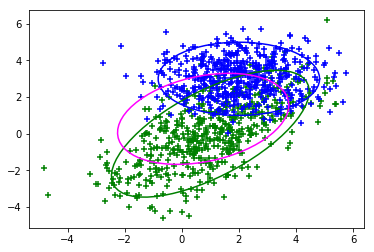
\includegraphics{images/fig2-3-2.png}
\caption{Example of a possible result}
\end{figure}

Fig. 2: Product of two pdfs (in blue and green)

    \begin{tcolorbox}[breakable, size=fbox, boxrule=1pt, pad at break*=1mm,colback=cellbackground, colframe=cellborder]
\prompt{In}{incolor}{22}{\boxspacing}
\begin{Verbatim}[commandchars=\\\{\}]
\PY{k}{def} \PY{n+nf}{bidimensional\PYZus{}gaussians\PYZus{}product}\PY{p}{(}\PY{n}{mean1}\PY{p}{,}\PY{n}{sigma1}\PY{p}{,}\PY{n}{mean2}\PY{p}{,}\PY{n}{sigma2}\PY{p}{,}\PY{n}{n\PYZus{}samples}\PY{p}{)}\PY{p}{:}

    \PY{n}{fig}\PY{p}{,} \PY{n}{ax} \PY{o}{=} \PY{n}{plt}\PY{o}{.}\PY{n}{subplots}\PY{p}{(}\PY{p}{)}
    
    \PY{c+c1}{\PYZsh{} Build the normal distributions}
    \PY{n}{pdf1} \PY{o}{=} \PY{n}{stats}\PY{o}{.}\PY{n}{multivariate\PYZus{}normal}\PY{p}{(}\PY{n}{mean1}\PY{o}{.}\PY{n}{flatten}\PY{p}{(}\PY{p}{)}\PY{p}{,} \PY{n}{sigma1}\PY{p}{)}
    \PY{n}{pdf2} \PY{o}{=} \PY{n}{stats}\PY{o}{.}\PY{n}{multivariate\PYZus{}normal}\PY{p}{(}\PY{n}{mean2}\PY{o}{.}\PY{n}{flatten}\PY{p}{(}\PY{p}{)}\PY{p}{,} \PY{n}{sigma2}\PY{p}{)}

    \PY{c+c1}{\PYZsh{} Generate n\PYZus{}samples }
    \PY{n}{rvs1} \PY{o}{=} \PY{n}{pdf1}\PY{o}{.}\PY{n}{rvs}\PY{p}{(}\PY{n}{n\PYZus{}samples}\PY{p}{)}
    \PY{n}{rvs2} \PY{o}{=} \PY{n}{pdf2}\PY{o}{.}\PY{n}{rvs}\PY{p}{(}\PY{n}{n\PYZus{}samples}\PY{p}{)}
    
    \PY{c+c1}{\PYZsh{} Draw the samples}
    \PY{n}{plt}\PY{o}{.}\PY{n}{scatter}\PY{p}{(}\PY{n}{rvs1}\PY{p}{[}\PY{p}{:}\PY{p}{,}\PY{l+m+mi}{0}\PY{p}{]}\PY{p}{,} \PY{n}{rvs1}\PY{p}{[}\PY{p}{:}\PY{p}{,}\PY{l+m+mi}{1}\PY{p}{]}\PY{p}{,} \PY{n}{marker}\PY{o}{=}\PY{l+s+s1}{\PYZsq{}}\PY{l+s+s1}{+}\PY{l+s+s1}{\PYZsq{}}\PY{p}{,} \PY{n}{color}\PY{o}{=}\PY{l+s+s1}{\PYZsq{}}\PY{l+s+s1}{green}\PY{l+s+s1}{\PYZsq{}}\PY{p}{)}
    \PY{n}{plt}\PY{o}{.}\PY{n}{scatter}\PY{p}{(}\PY{n}{rvs2}\PY{p}{[}\PY{p}{:}\PY{p}{,}\PY{l+m+mi}{0}\PY{p}{]}\PY{p}{,} \PY{n}{rvs2}\PY{p}{[}\PY{p}{:}\PY{p}{,}\PY{l+m+mi}{1}\PY{p}{]}\PY{p}{,} \PY{n}{marker}\PY{o}{=}\PY{l+s+s1}{\PYZsq{}}\PY{l+s+s1}{+}\PY{l+s+s1}{\PYZsq{}}\PY{p}{,} \PY{n}{color}\PY{o}{=}\PY{l+s+s1}{\PYZsq{}}\PY{l+s+s1}{blue}\PY{l+s+s1}{\PYZsq{}}\PY{p}{)}
   
    \PY{c+c1}{\PYZsh{} Calculate average of distributions}
    \PY{n}{invs1} \PY{o}{=} \PY{n}{linalg}\PY{o}{.}\PY{n}{inv}\PY{p}{(}\PY{n}{sigma1}\PY{p}{)} \PY{c+c1}{\PYZsh{} Hint use linalg.inv}
    \PY{n}{invs2} \PY{o}{=} \PY{n}{linalg}\PY{o}{.}\PY{n}{inv}\PY{p}{(}\PY{n}{sigma2}\PY{p}{)}

    \PY{n}{sigma3} \PY{o}{=} \PY{n}{linalg}\PY{o}{.}\PY{n}{inv}\PY{p}{(}\PY{n}{invs1}\PY{o}{+}\PY{n}{invs2}\PY{p}{)}
    \PY{n}{mean3} \PY{o}{=} \PY{n}{sigma3}\PY{o}{@}\PY{p}{(}\PY{p}{(}\PY{n}{invs2}\PY{n+nd}{@mean1}\PY{p}{)} \PY{o}{+} \PY{p}{(}\PY{n}{invs1}\PY{n+nd}{@mean2}\PY{p}{)}\PY{p}{)}  \PY{c+c1}{\PYZsh{} Hint: use the @ operator}

    \PY{c+c1}{\PYZsh{} Plot the ellipses}
    \PY{n}{mult} \PY{o}{=} \PY{l+m+mi}{2}
    \PY{n}{PlotEllipse}\PY{p}{(}\PY{n}{fig}\PY{p}{,} \PY{n}{ax}\PY{p}{,} \PY{n}{mean1}\PY{p}{,} \PY{n}{sigma1}\PY{p}{,} \PY{n}{mult}\PY{p}{,} \PY{n}{color}\PY{o}{=}\PY{l+s+s1}{\PYZsq{}}\PY{l+s+s1}{green}\PY{l+s+s1}{\PYZsq{}}\PY{p}{)}
    \PY{n}{PlotEllipse}\PY{p}{(}\PY{n}{fig}\PY{p}{,} \PY{n}{ax}\PY{p}{,} \PY{n}{mean2}\PY{p}{,} \PY{n}{sigma2}\PY{p}{,} \PY{n}{mult}\PY{p}{,} \PY{n}{color}\PY{o}{=}\PY{l+s+s1}{\PYZsq{}}\PY{l+s+s1}{blue}\PY{l+s+s1}{\PYZsq{}}\PY{p}{)}
    \PY{n}{PlotEllipse}\PY{p}{(}\PY{n}{fig}\PY{p}{,} \PY{n}{ax}\PY{p}{,} \PY{n}{mean3}\PY{p}{,} \PY{n}{sigma3}\PY{p}{,} \PY{n}{mult}\PY{o}{*}\PY{l+m+mf}{1.5}\PY{p}{,} \PY{n}{color}\PY{o}{=}\PY{l+s+s1}{\PYZsq{}}\PY{l+s+s1}{magenta}\PY{l+s+s1}{\PYZsq{}}\PY{p}{)} 
\end{Verbatim}
\end{tcolorbox}

    \begin{tcolorbox}[breakable, size=fbox, boxrule=1pt, pad at break*=1mm,colback=cellbackground, colframe=cellborder]
\prompt{In}{incolor}{23}{\boxspacing}
\begin{Verbatim}[commandchars=\\\{\}]
\PY{n}{n\PYZus{}samples} \PY{o}{=} \PY{l+m+mi}{500}
\PY{n}{mean1} \PY{o}{=} \PY{n}{np}\PY{o}{.}\PY{n}{vstack}\PY{p}{(}\PY{p}{[}\PY{l+m+mi}{1}\PY{p}{,} \PY{l+m+mi}{0}\PY{p}{]}\PY{p}{)}
\PY{n}{sigma1} \PY{o}{=} \PY{n}{np}\PY{o}{.}\PY{n}{array}\PY{p}{(}\PY{p}{[}\PY{p}{[}\PY{l+m+mi}{3}\PY{p}{,} \PY{l+m+mi}{2}\PY{p}{]}\PY{p}{,} \PY{p}{[}\PY{l+m+mi}{2}\PY{p}{,} \PY{l+m+mi}{3}\PY{p}{]}\PY{p}{]}\PY{p}{)}
\PY{n}{mean2} \PY{o}{=} \PY{n}{np}\PY{o}{.}\PY{n}{vstack}\PY{p}{(}\PY{p}{[}\PY{l+m+mi}{2}\PY{p}{,} \PY{l+m+mi}{3}\PY{p}{]}\PY{p}{)}
\PY{n}{sigma2} \PY{o}{=} \PY{n}{np}\PY{o}{.}\PY{n}{array}\PY{p}{(}\PY{p}{[}\PY{p}{[}\PY{l+m+mi}{2}\PY{p}{,} \PY{l+m+mi}{0}\PY{p}{]}\PY{p}{,} \PY{p}{[}\PY{l+m+mi}{0}\PY{p}{,} \PY{l+m+mi}{1}\PY{p}{]}\PY{p}{]}\PY{p}{)}

\PY{n}{bidimensional\PYZus{}gaussians\PYZus{}product}\PY{p}{(}\PY{n}{mean1}\PY{p}{,}\PY{n}{sigma1}\PY{p}{,}\PY{n}{mean2}\PY{p}{,}\PY{n}{sigma2}\PY{p}{,}\PY{n}{n\PYZus{}samples}\PY{p}{)}
\end{Verbatim}
\end{tcolorbox}

    \begin{center}
    \adjustimage{max size={0.9\linewidth}{0.9\paperheight}}{output_43_0.pdf}
    \end{center}
    { \hspace*{\fill} \\}
    
    \hypertarget{linear-transformation-of-normal-rvs}{%
\subsubsection{Linear transformation of normal
RVs}\label{linear-transformation-of-normal-rvs}}

As we mentioned at the start of this unit, when we linearly transform a
gaussian random variable, the result is still a gaussian. This is a very
desirable property to have, as it allows us to operate normally, as long
as the functions are linear.

    \hypertarget{assignment-9-applying-linear-transformation-to-bidimensional-distributions}{%
\subsubsection{\texorpdfstring{\textbf{{ASSIGNMENT 9: Applying linear
transformation to bidimensional
distributions}}}{ASSIGNMENT 9: Applying linear transformation to bidimensional distributions}}\label{assignment-9-applying-linear-transformation-to-bidimensional-distributions}}

Using the previous samples \(x_1\), check that the transformation
\(x_5 = A*x_1 +b\) results in a normal dist.
\(N(A \mu_1+b, A \Sigma_1 A^T)\). Given the matrices \texttt{A} and
\texttt{b} in the code below.

\textbf{Example}

Example of the result at scale=2.5 and the values given below:

\begin{figure}
\centering
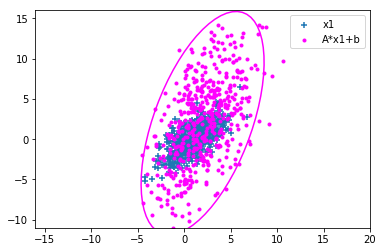
\includegraphics{images/fig2-3-3.png}
\caption{Example of a possible result}
\end{figure}

Fig. 3: Linear transformation of RVs. Original samples (in blue) and
results (in magenta)

    \begin{tcolorbox}[breakable, size=fbox, boxrule=1pt, pad at break*=1mm,colback=cellbackground, colframe=cellborder]
\prompt{In}{incolor}{24}{\boxspacing}
\begin{Verbatim}[commandchars=\\\{\}]
\PY{k}{def} \PY{n+nf}{linear\PYZus{}transform\PYZus{}demo}\PY{p}{(}\PY{n}{mean1}\PY{p}{,}\PY{n}{sigma1}\PY{p}{,}\PY{n}{mean2}\PY{p}{,}\PY{n}{sigma2}\PY{p}{,}\PY{n}{n\PYZus{}samples}\PY{p}{)}\PY{p}{:}
    
    \PY{n}{fig}\PY{p}{,} \PY{n}{ax} \PY{o}{=} \PY{n}{plt}\PY{o}{.}\PY{n}{subplots}\PY{p}{(}\PY{p}{)}
    
    \PY{c+c1}{\PYZsh{} Define the linear transformation}
    \PY{n}{A} \PY{o}{=} \PY{n}{np}\PY{o}{.}\PY{n}{array}\PY{p}{(}\PY{p}{[}\PY{p}{[}\PY{o}{\PYZhy{}}\PY{l+m+mi}{1}\PY{p}{,} \PY{l+m+mi}{2}\PY{p}{]}\PY{p}{,} \PY{p}{[}\PY{l+m+mi}{2}\PY{p}{,} \PY{l+m+mf}{1.5}\PY{p}{]}\PY{p}{]}\PY{p}{)}
    \PY{n}{b} \PY{o}{=} \PY{n}{np}\PY{o}{.}\PY{n}{vstack}\PY{p}{(}\PY{p}{[}\PY{l+m+mi}{3}\PY{p}{,} \PY{l+m+mi}{0}\PY{p}{]}\PY{p}{)}

    \PY{c+c1}{\PYZsh{} Build distribution}
    \PY{n}{pdf1} \PY{o}{=} \PY{n}{stats}\PY{o}{.}\PY{n}{multivariate\PYZus{}normal}\PY{p}{(}\PY{n}{mean1}\PY{o}{.}\PY{n}{flatten}\PY{p}{(}\PY{p}{)}\PY{p}{,} \PY{n}{sigma1}\PY{p}{)}

    \PY{c+c1}{\PYZsh{} Draw samples from it}
    \PY{n}{rvs1} \PY{o}{=} \PY{n}{pdf1}\PY{o}{.}\PY{n}{rvs}\PY{p}{(}\PY{n}{n\PYZus{}samples}\PY{p}{)}\PY{o}{.}\PY{n}{T}

    \PY{c+c1}{\PYZsh{} Show the samples}
    \PY{n}{ax}\PY{o}{.}\PY{n}{set\PYZus{}xlim}\PY{p}{(}\PY{p}{(}\PY{o}{\PYZhy{}}\PY{l+m+mi}{16}\PY{p}{,} \PY{l+m+mi}{20}\PY{p}{)}\PY{p}{)}
    \PY{n}{ax}\PY{o}{.}\PY{n}{set\PYZus{}ylim}\PY{p}{(}\PY{p}{(}\PY{o}{\PYZhy{}}\PY{l+m+mi}{11}\PY{p}{,} \PY{l+m+mi}{16}\PY{p}{)}\PY{p}{)}
    \PY{n}{ax}\PY{o}{.}\PY{n}{scatter}\PY{p}{(}\PY{n}{rvs1}\PY{p}{[}\PY{l+m+mi}{0}\PY{p}{,}\PY{p}{:}\PY{p}{]}\PY{p}{,} \PY{n}{rvs1}\PY{p}{[}\PY{l+m+mi}{1}\PY{p}{,}\PY{p}{:}\PY{p}{]}\PY{p}{,} \PY{n}{marker}\PY{o}{=}\PY{l+s+s1}{\PYZsq{}}\PY{l+s+s1}{+}\PY{l+s+s1}{\PYZsq{}}\PY{p}{,} \PY{n}{label}\PY{o}{=}\PY{l+s+s2}{\PYZdq{}}\PY{l+s+s2}{x1}\PY{l+s+s2}{\PYZdq{}}\PY{p}{)}

    \PY{c+c1}{\PYZsh{} Apply linear transformation transformacion lineal}
    \PY{n}{x5} \PY{o}{=} \PY{n}{A}\PY{n+nd}{@rvs1}\PY{o}{+}\PY{n}{b} \PY{c+c1}{\PYZsh{} Hint: use the @ operator}

    \PY{c+c1}{\PYZsh{} Show the new samples and its ellipse}
    \PY{n}{ax}\PY{o}{.}\PY{n}{scatter}\PY{p}{(}\PY{n}{x5}\PY{p}{[}\PY{l+m+mi}{0}\PY{p}{,}\PY{p}{:}\PY{p}{]}\PY{p}{,} \PY{n}{x5}\PY{p}{[}\PY{l+m+mi}{1}\PY{p}{,}\PY{p}{:}\PY{p}{]}\PY{p}{,} \PY{n}{marker}\PY{o}{=}\PY{l+s+s1}{\PYZsq{}}\PY{l+s+s1}{.}\PY{l+s+s1}{\PYZsq{}}\PY{p}{,} \PY{n}{color}\PY{o}{=}\PY{l+s+s1}{\PYZsq{}}\PY{l+s+s1}{magenta}\PY{l+s+s1}{\PYZsq{}}\PY{p}{,} \PY{n}{label}\PY{o}{=}\PY{l+s+s1}{\PYZsq{}}\PY{l+s+s1}{A*x1+b}\PY{l+s+s1}{\PYZsq{}}\PY{p}{)}
    \PY{n}{PlotEllipse}\PY{p}{(}\PY{n}{fig}\PY{p}{,} \PY{n}{ax}\PY{p}{,} \PY{n}{A}\PY{n+nd}{@mean1}\PY{o}{+}\PY{n}{b}\PY{p}{,} \PY{n}{A}\PY{n+nd}{@sigma1}\PY{n+nd}{@A}\PY{o}{.}\PY{n}{T}\PY{p}{,} \PY{l+m+mf}{2.5}\PY{p}{,} \PY{n}{color}\PY{o}{=}\PY{l+s+s1}{\PYZsq{}}\PY{l+s+s1}{magenta}\PY{l+s+s1}{\PYZsq{}}\PY{p}{)}
    \PY{n}{ax}\PY{o}{.}\PY{n}{legend}\PY{p}{(}\PY{p}{)}
\end{Verbatim}
\end{tcolorbox}

    \begin{tcolorbox}[breakable, size=fbox, boxrule=1pt, pad at break*=1mm,colback=cellbackground, colframe=cellborder]
\prompt{In}{incolor}{28}{\boxspacing}
\begin{Verbatim}[commandchars=\\\{\}]
\PY{n}{n\PYZus{}samples} \PY{o}{=} \PY{l+m+mi}{500}
\PY{n}{mean1} \PY{o}{=} \PY{n}{np}\PY{o}{.}\PY{n}{vstack}\PY{p}{(}\PY{p}{[}\PY{l+m+mi}{1}\PY{p}{,} \PY{l+m+mi}{0}\PY{p}{]}\PY{p}{)}
\PY{n}{sigma1} \PY{o}{=} \PY{n}{np}\PY{o}{.}\PY{n}{array}\PY{p}{(}\PY{p}{[}\PY{p}{[}\PY{l+m+mi}{3}\PY{p}{,} \PY{l+m+mi}{2}\PY{p}{]}\PY{p}{,} \PY{p}{[}\PY{l+m+mi}{2}\PY{p}{,} \PY{l+m+mi}{3}\PY{p}{]}\PY{p}{]}\PY{p}{)}
\PY{n}{mean2} \PY{o}{=} \PY{n}{np}\PY{o}{.}\PY{n}{vstack}\PY{p}{(}\PY{p}{[}\PY{l+m+mi}{2}\PY{p}{,} \PY{l+m+mi}{3}\PY{p}{]}\PY{p}{)}
\PY{n}{sigma2} \PY{o}{=} \PY{n}{np}\PY{o}{.}\PY{n}{array}\PY{p}{(}\PY{p}{[}\PY{p}{[}\PY{l+m+mi}{2}\PY{p}{,} \PY{l+m+mi}{0}\PY{p}{]}\PY{p}{,} \PY{p}{[}\PY{l+m+mi}{0}\PY{p}{,} \PY{l+m+mi}{1}\PY{p}{]}\PY{p}{]}\PY{p}{)}
    
\PY{n}{linear\PYZus{}transform\PYZus{}demo}\PY{p}{(}\PY{n}{mean1}\PY{p}{,}\PY{n}{sigma1}\PY{p}{,}\PY{n}{mean2}\PY{p}{,}\PY{n}{sigma2}\PY{p}{,}\PY{n}{n\PYZus{}samples}\PY{p}{)}
\end{Verbatim}
\end{tcolorbox}

    \begin{center}
    \adjustimage{max size={0.9\linewidth}{0.9\paperheight}}{output_47_0.pdf}
    \end{center}
    { \hspace*{\fill} \\}
    
    \hypertarget{student-discussion}{%
\subsection{Student discussion}\label{student-discussion}}

In the cell below, discuss what has been done in the notebook, what you
have found interesting, or any other relevant thought.

    { In the first block of the notebook, we evaluated a Gaussian
distribution using a range of values and \(\mu\) and \(\sigma\) values
of the Gaussian Distribution. Also in another assignment, we generated
random values from the Gaussian. With this function, we could draw a
Gaussian with these values. We also appreciated that as we take more
values, the ``precision'' of the graphic increases. }

{ In the second block, we verified some properties about the Gaussians,
like the ``Central Limit Theorem'', the ``product of a Gaussian is still
a Gaussian'' or the ``lineal transformation of a Gaussian is still a
Gaussian''. }

{ In the last block, we worked with multimdimensional distributiones: We
implemented the sum of RVs (Random Values) generated from Gaussians, the
product of two bidimensional Gaussians and finally we implemented a
function that apply linear transformation to bidimensional Gaussian
distributions. }


    % Add a bibliography block to the postdoc
    
    
    
\end{document}
